\graphicspath{{Ch4_2020_bmvc/figs/}}

\chapter{{Graph Density-Aware Losses for Novel Compositions in Scene Graph Generation}\label{ch:bmvc2020}}

%\chapter{PROLOGUE TO SECOND ARTICLE}
\section*{Prologue}
\addcontentsline{toc}{section}{Prologue}

% \begin{tabular}{p{0.16\linewidth}p{0.78\linewidth}}
%      \textit{Title:} & Graph Density-Aware Losses for Novel Compositions in Scene Graph Generation \\
%      \textit{Authors:} & Boris Knyazev, Harm de Vries, Cătălina Cangea, Graham Taylor, Aaron Courville, Eugene Belilovsky \\
%      \textit{Published at:} & \venue{British Machine Vision Conference (BMVC 2020)} \\
%     \textit{Code release:} & \url{https://github.com/bknyaz/sgg} \\
%     \textit{Personal contributions:} & developed the key components of algorithms and models; developed the code; designed
% and ran all experiments; wrote most of the article.
% \end{tabular}

\vspace{10pt}
\densepar{Context.}
Visual recognition models have been greatly improved across different applications largely due to the advances in convolutional neural networks (\cnns). Scene graph generation (SGG) is a task where objects and the relationships between them must be recognized from images~\citep{xu2017scene}. Many state of the art SGG models have tuned their performance for frequent compositions of objects and relationships~\citep{zellers2018neural}. Unfortunately, there is an extreme reduction in performance of these models on rare or unseen compositions~\citep{tang2020unbiased}. Understanding and addressing this problem in a realistic large-scale setup is challenging yet needed to increase the  practical value of SGG models.\looseness-1

\densepar{Contributions.}
We analyzed the loss function typically used to train SGG models and found that it ignores an important property of visual scene graphs --- graph density (number of edges \wrt the number of nodes). To address this issue, we developed a loss with terms that are normalized according to the graph density. The SGG models trained with our graph-density normalized loss significantly improve in generalization to rare and unseen compositions.

\densepar{Recent works.}
\citet{tang2020unbiased} proposed a method based on causal inference to ``debias'' SGG models and improve generalization. In line with our work, \citet{suhail2021energy} proposed an improved loss function based on energy defined on graphs. \citet{khandelwal2021segmentation} added more precise object representation in the form of segmentation masks that also improved compositional generalization. \citet{liu2021fully} proposed relation affinity fields to better generalize to unseen/rare compositions. While these approaches are applied to the SGG task, object-centric learning is a more general-purpose method that can potentially improve generalization in a larger variety of visual tasks~\citep{locatello2020object,dittadi2021generalization}.

\section{Introduction}

In recent years, there has been growing interest to connect successes in visual perception with language and reasoning~\citep{su2019vl,zhou2019unified}. This requires us to design systems that can not only recognize objects, but understand and reason about the relationships between them. 
This is essential for such tasks as visual question answering (VQA)~\citep{antol2015vqa,hudson2019gqa,cangea2019videonavqa} or caption generation~\citep{yang2019auto, gu2019unpaired}. 
However, predicting a high-level semantic output (\eg~answer) from a low-level visual signal (\eg~image) is challenging due to a vast gap between the modalities.
To bridge this gap, it would be useful to have some intermediate representation that can be relatively easily generated by the low-level module and, at the same time, can be effectively used by the high-level reasoning module.
We want this representation to semantically describe the visual scene in terms of objects and relationships between them, which leads us to a structured image representation, the \textbf{scene graph} (SG)~\citep{johnson2015image, Krishna_2017}.
A scene graph is a collection of visual relationship \textit{triplets}: <\textit{subject}, \textit{predicate}, \textit{object}> (\eg~<cup, on, table>). Each node in the graph corresponds to a subject or object (with a specific image location) and edges to predicates~(\fig{\ref{fig:overview}}). 
Besides bridging the gap, SGs can be used to verify how well the model has understood the visual world, as opposed to just exploiting one of the biases in a dataset~\citep{jabri2016revisiting,anand2018blindfold,bahdanau2018systematic}.
Alternative directions to SGs include, for example, attention~\citep{norcliffe2018learning} and neural-symbolic models~\citep{vedantam2019probabilistic}.\looseness-1

\begin{figure}[t]
	\centering
	\begin{scriptsize}
		\setlength{\tabcolsep}{1pt}
		\begin{tabular}{c} 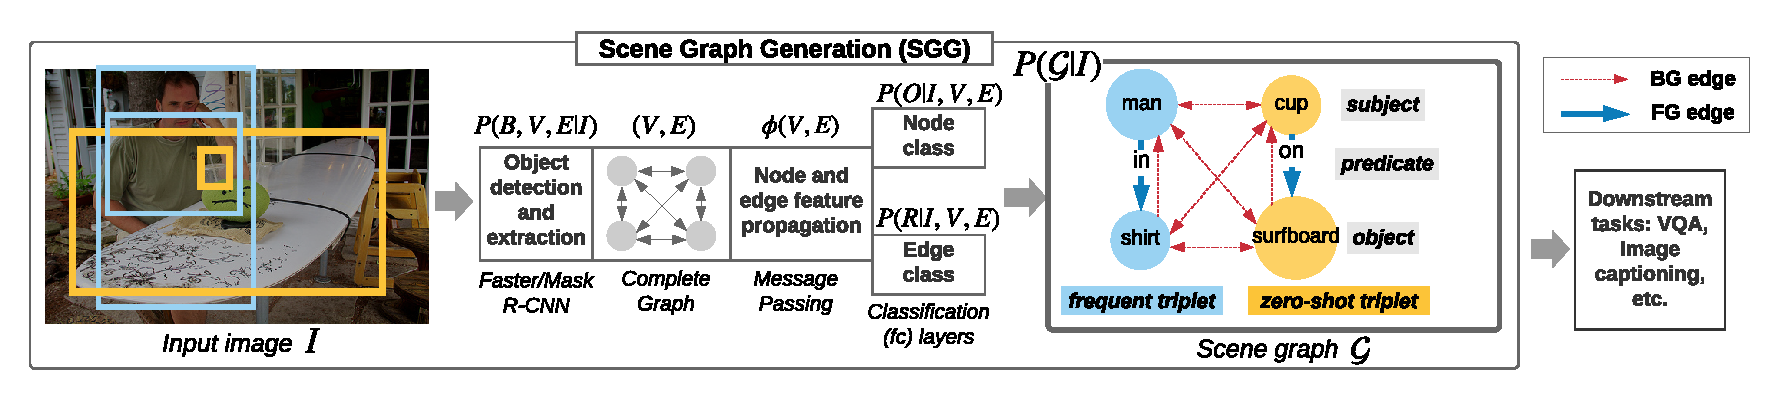
\includegraphics[width=0.99\textwidth,align=c,trim={0 0.2cm 0 0.2cm},clip]{cup_on_surfboard_overview1.pdf} \\
		\end{tabular}
	\end{scriptsize}
	\vspace{-5pt}
	\caption{\small In this work, we improve scene graph generation $P({\cal G} | I)$. In many downstream tasks, such as VQA, the result directly depends on the accuracy of predicted scene graphs.}
	\label{fig:overview}
\end{figure}

\begin{figure}
	\scriptsize
	\centering
	\setlength{\tabcolsep}{3pt}
	{
		\begin{minipage}{0.5\linewidth}
			\hspace{-20pt}
			\begin{tabular}{cc}
				\multicolumn{2}{c}{{\hspace{30pt}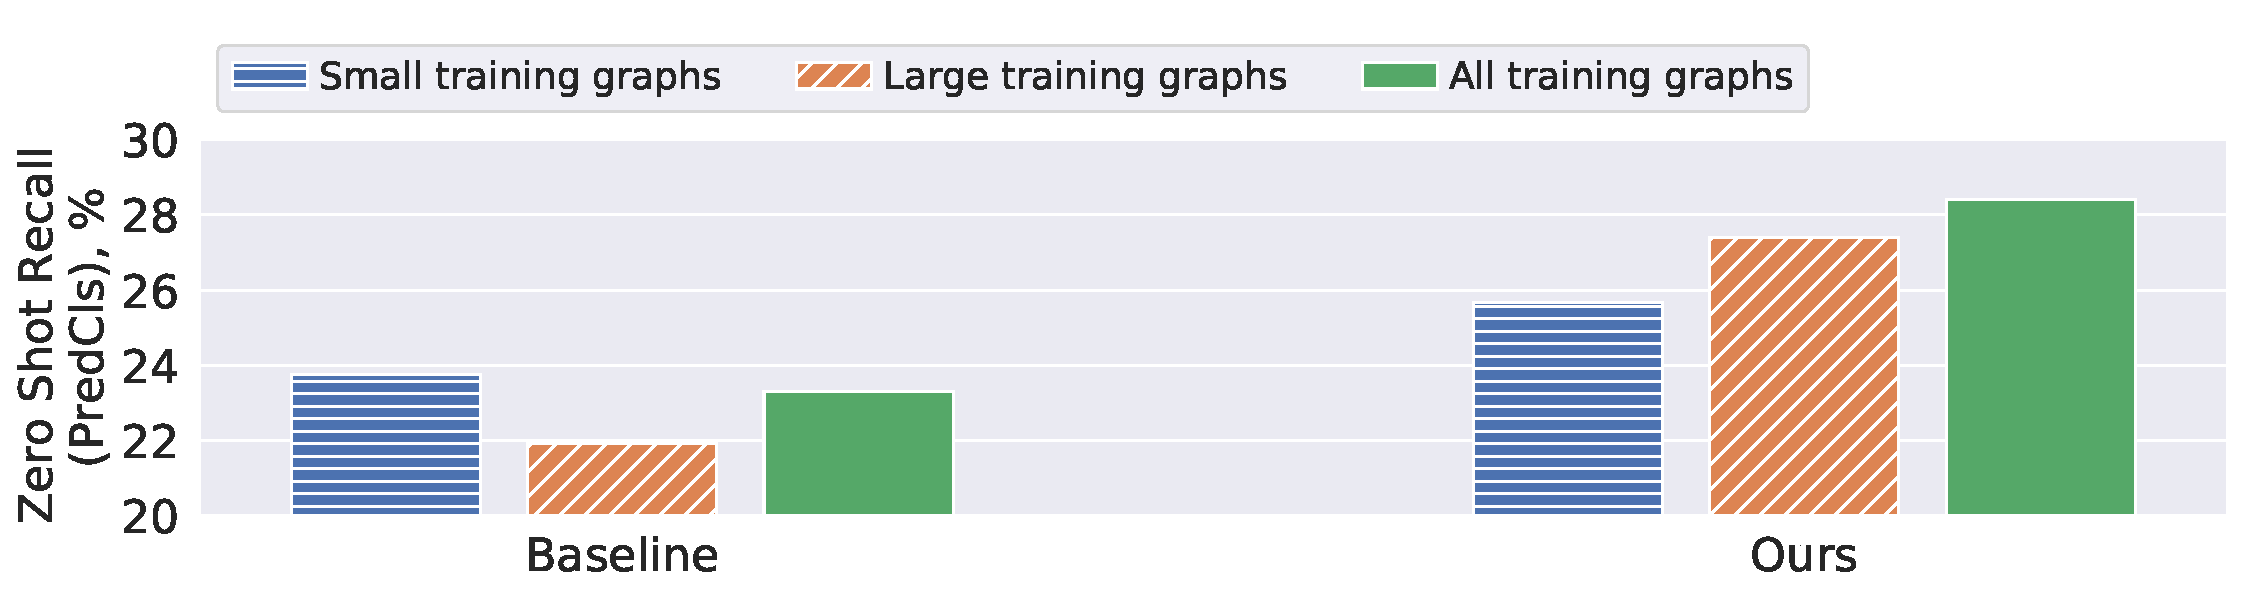
\includegraphics[width=0.95\textwidth,trim={3.5cm 8.3cm 7cm 0.8cm},clip]{legend.pdf}}} \vspace{-3pt} \\
				\vspace{-3pt}
				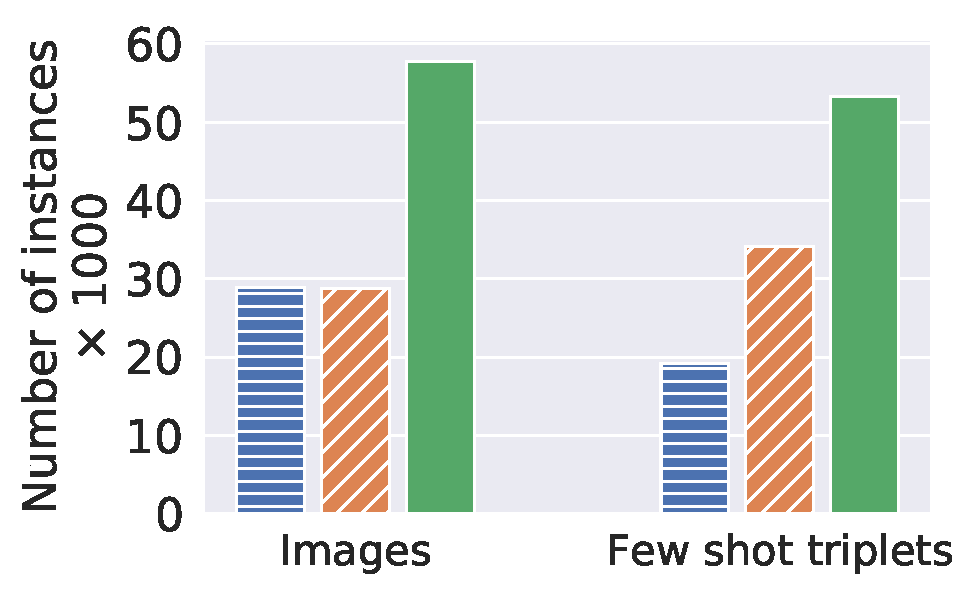
\includegraphics[align=c,height=2.7cm]{large_graphs_train_labels.pdf} &
				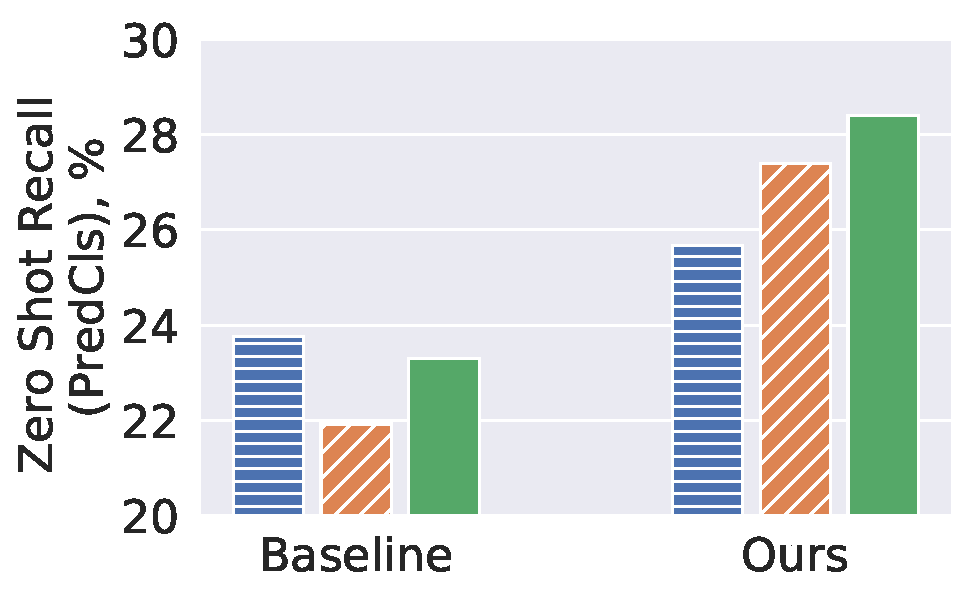
\includegraphics[align=c,height=2.7cm]{large_graphs_vs_recall_predcls_zs.pdf} \\
				\hspace{20pt} (a) & \hspace{20pt} (b) 
			\end{tabular}
		\end{minipage}
	}
	\hspace{10pt}
	{
		\begin{minipage}{0.4\linewidth}
			\vspace{8pt}
			\begin{tabular}{p{3cm}p{3cm}}
				\centering
				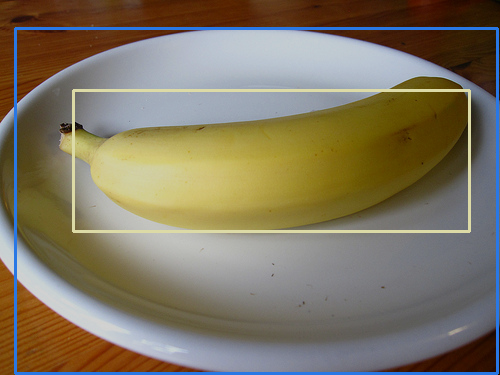
\includegraphics[height=2cm, align=c]{2409758_stanford_nolabel.png} & 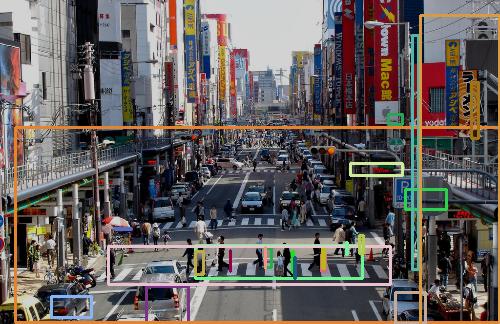
\includegraphics[height=2cm, align=c]{1160208_stanford_nolabel.png} \Bstrut \\ 
				\centering (c) Image with a small scene graph & \centering (d) Image with a large scene graph
			\end{tabular}
		\end{minipage}
	}
	\vspace{-3pt}
	\caption{\small \textbf{Motivation of our work.} We split the training set of Visual Genome~\citep{Krishna_2017} into two subsets: those with relatively small ($\leq 10$ nodes) and large ($>10$ nodes) graphs. (\textbf{a}) While each subset contains a similar number of images (the three left bars), larger graphs contain more few-shot labels (the three right bars). (\textbf{b}) Baseline methods (\citep{xu2017scene} in this case) fail to learn from larger graphs due to their loss function. However, training on large graphs and corresponding few-shot labels is important for stronger generalization. We address this limitation and significantly improve results on zero and few-shots. (\textbf{c, d}) Small and large scene graphs typically describe simple and complex scenes respectively. \looseness-1 
	}
	%\vspace{-10pt}
	\label{fig:motivation}
\end{figure}


\textbf{Scene graph generation} (SGG) is the task of predicting a SG given an input image. The inferred SG can be used directly for downstream tasks such as VQA~\citep{zhang2019empirical,NSM2019}, image captioning~\citep{yang2019auto, gu2019unpaired} or retrieval~\citep{johnson2015image,belilovsky2017joint,tang2020unbiased}.
A model which performs well on SGG should demonstrate the ability to ground visual concepts to images and generalize to compositions of objects and predicates in new contexts. In real world images, some compositions (\eg~<cup, on, table> ) appear more frequently than others (\eg~<cup, on, \textit{surfboard}> or <cup, \textit{under}, table>), which creates a strong frequency bias. This makes it particularly challenging for models to generalize to novel (zero-shot) and rare (few-shot) compositions, even though each of the subjects, objects and predicates have been observed at training time.
The problem is exacerbated by the test set and evaluation metrics, which do not penalize models that blindly rely on such bias. Indeed,~\citet{zellers2018neural} has pointed out that SGG models largely exploit simple co-occurrence information. In fact, the performance of models predicting solely based on frequency  (i.e. a cup is most likely to be \textit{on} a \textit{table}) is not far from the state-of-the-art using common metrics (see \textsc{Freq} in Table~\ref{table:main_results}).\looseness-1

In this work, we reveal that (a) the frequency bias exploited by certain  models leads to poor generalization on few-shot and zero-shot compositions; (b) existing models disproportionately penalize large graphs, even if these often contain many of the infrequent visual relationships, which leads to performance degradation on few and zero-shot cases (\fig{\ref{fig:motivation}}). We address these challenges and show that our suggested improvements can provide benefits for two strong baseline models~\citep{xu2017scene,zellers2018neural}. Overall, we make the following four \textbf{contributions}:

\begin{enumerate}[leftmargin=10pt,labelsep=2pt]
	\itemsep0em 
	\item \textbf{Improved loss}: we introduce a density-normalized edge loss, which improves results on all metrics, especially for few and zero-shots (\secref{\ref{sec:loss_norm}});
	\item \textbf{Novel weighted metric}: we illustrate several issues in the evaluation of few and zero-shots, proposing a novel weighted metric which can better track the performance of this critical desiderata (\secref{\ref{sec:metric}});
	\item \textbf{Frequency bias}: we demonstrate a negative effect of the frequency bias, proposed in Neural Motifs~\citep{zellers2018neural}, on few and zero-shot performance (\secref{\ref{sec:experiments}}); 
	\item \textbf{Scaling to GQA}: in addition to evaluating on Visual Genome (VG)~\citep{Krishna_2017}, we confirm the usefulness of our loss and metrics on GQA~\citep{hudson2019gqa} -- an improved version of VG. GQA has not been used to evaluate SGG models before and is interesting to study, because compared to VG its scene graphs are cleaner, larger, more dense and contain a larger variety of objects and predicates (\secref{\ref{sec:experiments}}).
\end{enumerate}
\vspace{-10pt}


\section{Related work}

\textbf{Zero-shot learning.}
In vision tasks, such as image classification, zero-shot learning has been extensively studied, and the main approaches are based on attributes~\citep{lampert2013attribute} and semantic embeddings~\citep{frome2013devise, xian2016latent}.
The first approach is related to the zero-shot problem we address in this work: it assumes that all individual attributes of objects (color, shape, etc.) are observed during training, such that novel classes can be detected at test time based on \textit{compositions} of their attributes.
Zero-shot learning in scene graphs is similar: all individual subjects, objects and predicates are observed during training, but most of their compositions are not. This task was first evaluated in~\citep{lu2016visual} on the VRD dataset using a joint vision-language model. 
Several follow-up works attempted to improve upon it: by learning a translation operator in the embedding space~\citep{zhang2017visual}, clustering in a weakly-supervised fashion~\citep{peyre2017weakly}, using conditional random fields~\citep{cong2018scene} or optimizing a cycle-consistency loss to learn object-agnostic features~\citep{yang2018shuffle}.
Augmentation using generative networks to generate more examples of rare cases is another promising approach~\citep{wang2019generating}; but, it was only evaluated in the predicate classification task. In our work, we also consider subject/object classification to enable the classification of the whole triplets, making the ``image to scene graph'' pipeline complete. Most recently,~\citet{tang2020unbiased} proposed learning causal graphs and showed strong performance in zero-shot cases.

While these works improve generalization, none of them has identified the challenges and importance of learning from large graphs for generalization. By concentrating the model's capacity on smaller graphs and neglecting larger graphs, baseline models limit the variability of training data, useful for stronger generalization~\citep{hill2019environmental}. Our loss enables this learning, increasing the effective data variability. Moreover, previous gains typically incur a large computational cost, while our loss has negligible cost and can be easily added to other models.\looseness-1


\textbf{Few-shot predicates.} 
Several recent works have addressed the problem of imbalanced and few-shot predicate classes ~\citep{chen2019knowledge, dornadula2019visual,tang2019learning,zhang2019graphical,tang2020unbiased,chen2019scene}. However, compared to our work, these works have not considered the imbalance between foreground and background edges, which is more severe than other predicate classes (\fig{\ref{fig:pred_distr}}) and is important to be fixed as we show in this work.
Moreover, we argue that the compositional generalization, not addressed in those works, can be more difficult than generalization to rare predicates. For example, the triplet <cup, on, surfboard> is challenging to be predicted correctly as a whole; even though `on' can be the most frequent predicate, it has never been observed together with `cup' and `surfboard'. Experimental results in previous work~\citep{lu2016visual,zhang2017visual,yang2018shuffle,wang2019generating,tang2020unbiased} highlight this difficulty. Throughout this work, by ``few-shot'' we assume triplets, not predicates.

\textbf{``Unbiasing'' methods.}
Our idea is similar to the Focal loss~\citep{lin2017focal}, which addresses the imbalance between foreground and background objects in the object detection task. However, directly applying the focal loss to Visual Genome is challenging, due to the large amount of missing and mislabeled examples in the dataset. In this case, concentrating the model's capacity on ``hard'' examples can be equivalent to putting more weight on noise, which can hurt performance. \citet{tang2020unbiased} compared the focal loss and other unbiasing methods, such as upsampling and upweighting, and did not report significantly better results.


\section{Methods}
\label{sec:methods}
In this section, we will review a standard loss used to train scene graph generation models (\secref{\ref{sec:baseline}}) and describe our improved loss (\secref{\ref{sec:loss_norm}}). We will then discuss issues with evaluating rarer combinations and propose a new weighted metric (\secref{\ref{sec:metric}}). 



\subsection{Overview of scene graph generation}
\label{sec:baseline}
In scene graph generation, given an image $I$, we aim to output a scene graph ${\cal G}=(O,R)$ consisting of a set of subjects and objects ($O$) as nodes and a set of relationships or predicates ($R$) between them as edges (\fig{\ref{fig:overview}}). So the task is to maximize the probability $P({\cal G} | I)$, which can be expressed as  $P(O,R | I) = P(O |I)\ P(R | I,O)$.
Except for works that directly learn from pixels~\citep{newell2017pixels}, the task is commonly~\citep{xu2017scene,yang2018graph,zellers2018neural} reformulated by first detecting bounding boxes $B$ and extracting corresponding object and edge features, $V=f(I,B)$ and $E=g(I,B)$ respectively, using some functions $f,g$ (\eg~a ConvNet followed by ROI Align~\citep{he2017mask}):
\begin{equation}
\label{eq:scene_graph_prob_box}
P({\cal G} |I) = P(V,E |I)\ P(O,R | V,E,I).%
\end{equation}
The advantage of this approach is that solving $P(O,R | V,E,I)$ is easier than solving $P(O,R | I)$. At the same time, to compute $P(V,E |I)$ we can use pretrained object detectors~\citep{ren2015faster, he2017mask}.
Therefore, we follow~\citep{xu2017scene,yang2018graph,zellers2018neural} and use this approach to scene graph generation.

In practice, we can assume that the pretrained object detector is fixed or that ground truth bounding boxes $B$ are available, so we can assume $P(V,E|I)$ is constant. In addition, following~\citep{lu2016visual,xu2017scene,yang2018graph}, we can assume conditional independence of variables $O$ and $R$: $P(O,R|V,E,I)=P(O|V,E,I)P(R|V,E,I)$. We thus obtain the scene graph generation loss:
\begin{equation}
\label{eq:scene_graph_prob_simple}
-\text{log} P({\cal G} |I) = -\text{log} P(O | V,E,I) - \text{log} P(R | V,E,I).
\end{equation}
Some models~\citep{zellers2018neural,zhang2019graphical} do not assume the conditional independence of $O$ and $R$, making predicates explicitly depend on subject and object labels: $P(O,R|V,E,I)=P(O|V,E,I) P(R|O,V,E,I)$. However, such a model must be carefully regularized, since it can start to ignore $(V,E,I)$ and mainly rely on the frequency distribution $P(R|O)$ as a stronger signal. For example, the model can learn that between `cup' and `table' the relationship is most likely to be `on', regardless the visual signal. As we show, this can hurt generalization.\looseness-1

\begin{wrapfigure}{r}{5.7cm}%
	\vspace{-10pt}
	\centering
	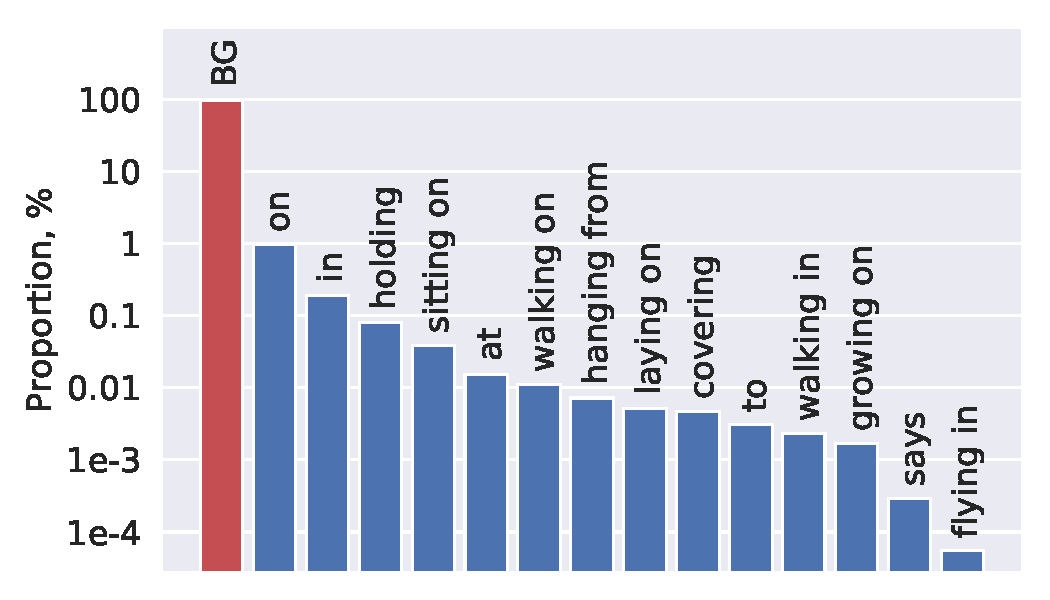
\includegraphics[width=5.5cm,align=c]{rel_distr_train_VG.pdf} \\
	\vspace{-5pt}
	\caption{\small Predicate distribution in Visual Genome (split~\citep{xu2017scene}). BG edges (note the log scale) dominate, with >96\% of all edges, creating an extreme imbalance. For clarity, only some most and least frequent predicate classes are shown.\looseness-1}
	\label{fig:pred_distr}
	%\vspace{-20pt}
\end{wrapfigure}

\eqref{eq:scene_graph_prob_simple} is commonly handled as a multitask classification problem, where each task is optimized by the cross-entropy loss ${\cal L}$.
In particular, given a batch of scene graphs with $N$ nodes and $M$ edges in total, the loss is the following:
\begin{equation}
\label{eq:loss_baseline}
{\cal L} = {\cal L}_{node} + {\cal L}_{edge} = \frac{1}{N}\sum_i^N{\cal L}_{obj,i} + \frac{1}{M}\sum_{ij}^M {\cal L}_{rel,ij}.
\end{equation}
Node and edge features $(V,E)$ output by the detector form a complete graph without self-loops (\fig{\ref{fig:overview}}). So, conventionally~\citep{xu2017scene,yang2018graph,zellers2018neural}, the loss is applied to all edges: $M \approx N^2$.
These edges can be divided into foreground (FG), corresponding to annotated edges, and background (BG), corresponding to not annotated edges: $M = M_{FG} + M_{BG}$.
The BG edge type is similar to a ``negative'' class in the object detection task and has a similar purpose.
Without training on BG edges, at test time the model would label all pairs of nodes as ``positive'', i.e. having some relationship, when often it is not the case (at least, given the vocabulary in the datasets). Therefore, not using the BG type can hurt the quality of predicted scene graphs and can lower recall.\looseness-1

\subsection{Hyperparameter-free normalization of the edge loss}
\label{sec:loss_norm}

\textbf{Baseline loss as a function of graph density.}
In scene graph datasets such as Visual Genome, the number of BG edges is greater than FG ones (\fig{\ref{fig:pred_distr}}), yet the baseline loss~\eqref{eq:loss_baseline} does not explicitly differentiate between BG and other edges. If we assume a fixed probability for two objects to have a relationship, then as the number of nodes grows we can expect fewer of them to have a relationship. Thus the graph density can vary based on the number of nodes (\fig{\ref{fig:graph_density}}), a fact not taken into account in \eqref{eq:loss_baseline}.
To avoid this, we start by decoupling the edge term of~\eqref{eq:loss_baseline} into the foreground (FG) and background (BG) terms:\looseness-1
%
\begin{equation}
{\cal L}_{edge} = \frac{1}{M}\sum_{ij}^M{\cal L}_{rel,ij} =  \frac{1}{M_{FG} + M_{BG}} \bigg[ \underbrace{\sum\nolimits_{ij \in \cal E}^{M_{FG}}{\cal L}_{rel,ij}}_{\text{FG edges}} + \underbrace{\sum\nolimits_{ij \notin \cal E}^{M_{BG}}{\cal L}_{rel,ij}}_{\text{BG edges}} \bigg]  ,
\end{equation}
%
\noindent where ${\cal E}$ is a set of FG edges, $M_{FG}$ is the number of FG edges ($|{\cal E}|$) and $M_{BG}$ is the number of BG edges.
Next, we denote FG and BG edge losses averaged per batch as ${\cal L}_{FG}=1/M_{FG}\sum_{ij \in \cal E}^{M_{FG}}{\cal L}_{rel,ij}$ and ${\cal L}_{BG}=1/M_{BG}\sum_{ij \notin \cal E}^{M_{BG}}{\cal L}_{rel,ij}$, respectively.
Then, using the definition of graph density as a proportion of FG edges to all edges, $d=M_{FG} / (M_{BG} + M_{FG})$, we can express the total baseline loss equivalent to \eqref{eq:loss_baseline} \textbf{as a function of graph density}:\looseness-1
%
\begin{equation}
\label{eq:loss_decouple}
\boxed{
	{\cal L} = {\cal L}_{node} + d {\cal L}_{FG}  + (1 - d) {\cal L}_{BG}.}
\end{equation}


\noindent\textbf{Density-normalized edge loss.}
\eqref{eq:loss_decouple} and \fig{\ref{fig:graph_density}} allow us to notice two issues:

\begin{enumerate}[leftmargin=10pt,labelsep=2pt]%
	\itemsep0em 
	\item \textbf{Discrepancy of the loss between graphs of different sizes.} Since $d$ exponentially decreases with graph size (~\ref{fig:graph_density}, left), FG edges of larger graphs are weighted less than edges of smaller graphs in the loss (\fig{\ref{fig:graph_density}}, middle), making the model neglect larger graphs.\looseness-1
	
	\item \textbf{Discrepancy between object and edge losses.}
	Due to $d$ tending to be small on average, $L_{edge}$ is much smaller than $L_{node}$, so the model might focus mainly on $L_{node}$ (\fig{\ref{fig:graph_density}}, right).\looseness-1
\end{enumerate}

\vspace{-5pt}
Both issues can be addressed by normalizing FG and BG terms by graph density $d$:
\begin{equation}
\label{eq:loss_norm}
\boxed{{\cal L} = {\cal L}_{node} + \gamma \big[ {\cal L}_{FG}  + {M_{BG}}/{M_{FG}} {\cal L}_{BG}\big].}
\end{equation}
\noindent where $\gamma=1$ in our default hyperparameter-free variant and $\gamma \neq 1$ only to empirically analyze the loss (Table~\ref{table:loss_ablations}). Even though the BG term still depends on graph density, we found it to be less sensitive to variations in $d$, since the BG loss quickly converges to some stable value, performing a role of regularization (\fig{\ref{fig:graph_density}}, right).
We examine this in detail in \secref{\ref{sec:experiments}}.

\begin{figure}%[h]
	\centering
	\begin{small}
		\setlength{\tabcolsep}{1pt}
		\begin{tabular}{ccc}
			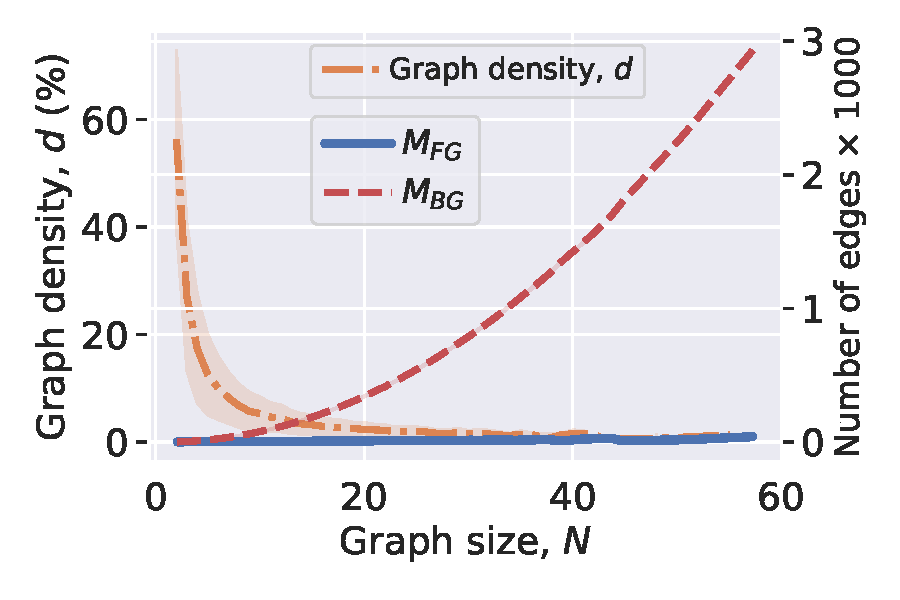
\includegraphics[width=0.3\textwidth,align=c]{VG_graphs_bg_b1.pdf} &
			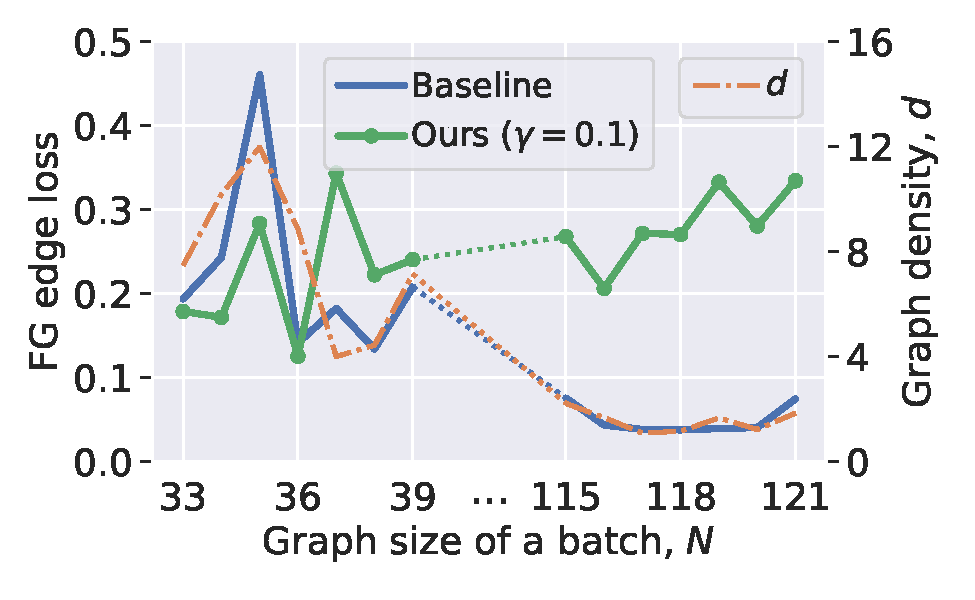
\includegraphics[width=0.3\textwidth,align=c]{loss_adaptive4_b6_graphsize.pdf} & 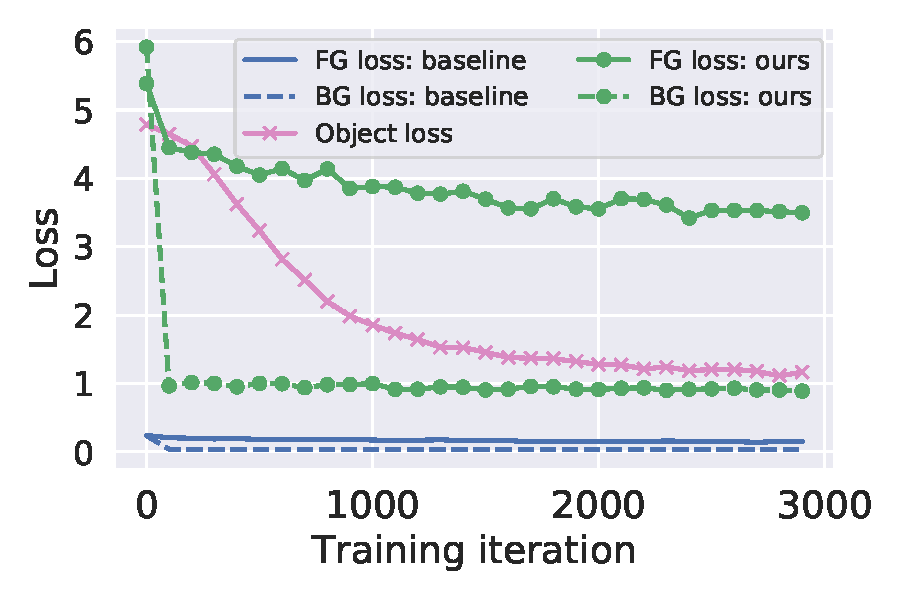
\includegraphics[width=0.3\textwidth,align=c]{losses_vs_iter_loss_adaptive4_b6.pdf} \\ $d \rightarrow 0 $ for large graphs & Large graphs are downweighted by $d$ & $L_{edge} \ll L_{node}$ \\
		\end{tabular}
	\end{small}
	%\vspace{-5pt}
	\caption{
		\small (\textbf{left}) The number of FG edges grows much more slowly with graph size than the number of BG edges (on VG: $M_{FG}\approx 0.5N$). This leads to: (\textbf{middle}) Downweighting of the FG loss on larger graphs and effectively limiting the amount and variability of training data, since large graphs contain a lot of labeled data (\fig{\ref{fig:motivation}}); here, losses of converged models for batches sorted by graph size are shown. (\textbf{right}) Downweighting of the edge loss $L_{edge}$ overall compared to $L_{node}$, even though both tasks are equally important to correctly predicting a scene graph. Our normalization fixes both issues.}
	\label{fig:graph_density}
\end{figure}

\subsection{Weighted triplet recall}
\label{sec:metric}

The common evaluation metric for scene graph prediction is image-level Recall@K or R@K \citep{xu2017scene, yang2018graph, zellers2018neural}.
To compute it, we first need to extract the top-$K$ triplets, $\text{Top}_K$, from the \textit{entire image} based on ranked predictions of a model . Given a set of ground truth triplets, \text{GT}, the image-level R@K is computed as (see \fig{\ref{fig:eval}} for a visualization): 
%\setlength{\abovedisplayskip}{3pt}
%\setlength{\belowdisplayskip}{3pt}
\begin{equation}
\label{eq:recall_image}
\text{R}@\text{K} = {|\text{Top}_K \cap \text{GT}|}/{|\text{GT}|}.
\end{equation}
There are four issues with this metric:
%(we discuss additional details in~\apdx):

\begin{enumerate}[label=(\alph*),wide, labelindent=0pt, leftmargin=0pt, listparindent=0pt, labelsep=3pt]
	\itemsep0em 
	\item The frequency bias of triplets means more frequent triplets will dominate the metric.
	\item The denominator in~\eqref{eq:recall_image} creates discrepancies between images with different $|\text{GT}|$ (the number of ground truth triplets in an image), especially pronounced in few/zero shots.
	\item Evaluation of zero ($n=0$) and different few-shot cases $n=1,5,10,...$~\citep{wang2019generating} leads to many R@K results~\citep{wang2019generating}. This complicates the analysis. Instead, we want a single metric for all $n$.
	\item Two ways of computing the image-level recall~\citep{newell2017pixels,zellers2018neural}, graph \textit{constrained} and \textit{unconstrained}, lead to very different results and complicate the comparison (\fig{\ref{fig:eval}}).%
\end{enumerate}

To address issue \textbf{(a)}, the predicate-normalized metric, mean recall (mR@K)~\citep{chen2019knowledge,tang2019learning} and weighted mR@K were introduced~\citep{zhang2019graphical}. These metrics, however, only address the imbalance of predicate classes, not whole triplets.
Early work~\citep{lu2016visual,dai2017detecting} used triplet-level Recall@K (or R$_{tr}$@K) for some tasks (\eg~predicate detection), which is based on ranking predicted triplets for each ground truth subject-object pair independently; the pairs without relationships are not evaluated. Hence, R$_{tr}$@K is similar to top-$K$ accuracy.
This metric avoids issues \textbf{(b)} and \textbf{(d)}, but the issues of the frequency bias \textbf{(a)} and unseen/rare cases \textbf{(c)} still remain.
To alleviate these, we adapt this metric to better track unseen and rare cases. We call our novel metric Weighted Triplet Recall wR$_{tr}$@K, which computes a recall at each triplet and reweights the average result based on the frequency of the GT triplet in the training set: 
%\setlength{\abovedisplayskip}{3pt}
%\setlength{\belowdisplayskip}{3pt}
\begin{equation}
\label{eq:recall_triplet}
\text{wR}_{tr}@\text{K} =  \sum\nolimits_t^T w_t [\text{rank}_t \leq K],
\end{equation}
\noindent where $T$ is the number of all test triplets, $[\cdot]$ is the Iverson bracket, $w_t=\frac{1}{(n_t + 1)\sum_t 1/(n_t + 1)} \in [0,1]$ and $n_t$ is the number of occurrences of triplet $t$ in the training set; $n_t + 1$ is used to handle zero-shot triplets; $\sum_t w_t = 1$. Since wR$_{tr}$@K is still a triplet-level metric, we avoid issues \textbf{(b)} and \textbf{(d)}. Our metric is also robust to the frequency-bias \textbf{(a)}, since frequent triplets (with high $n_t$) are downweighted proportionally, which we confirm by evaluating the \textsc{Freq} model from~\citep{zellers2018neural}. Finally, a single wR$_{tr}$@K value shows zero and few-shot performance linearly aggregated for all $n \geq 0$, solving issue \textbf{(c)}. 

\begin{figure}%[h]
	\centering
% 	\vspace{-10pt}
	{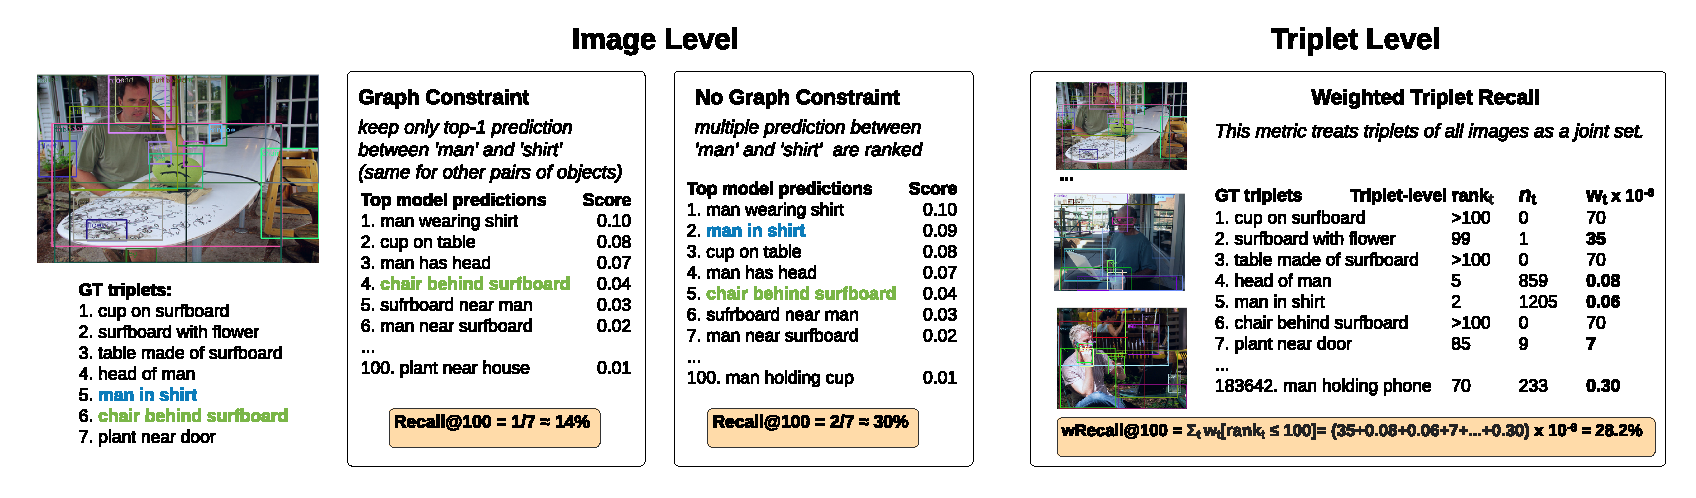
\includegraphics[width=\textwidth]{metrics.pdf}}
	\vspace{-10pt}
	\caption{\small Existing image-level recall metrics \textit{versus} our proposed weighted triplet recall. We first make unweighted predictions $\text{rank}_t \leq K$ for all GT triplets in all test images, then reweight them according to the frequency distribution~\eqref{eq:recall_triplet}. Computing our metric per image would be noisy.
	}
	\label{fig:eval}
\end{figure}

\vspace{-5pt}
\section{Experiments}
\label{sec:experiments}
\vspace{-5pt}

\textbf{Datasets.}
We evaluate our loss and metric on Visual Genome~\citep{Krishna_2017}. Since it is a noisy dataset, several ``clean'' variants were introduced. We mainly experiment with the most common variant (VG)~\citep{xu2017scene}, which consists of the 150 most frequent object and 50 predicates classes. An alternative variant (VTE)~\citep{zhang2017visual} has been often used for zero-shot evaluation. Surprisingly, we found that the VG split~\citep{xu2017scene} is better suited for this task, given a larger variability of zero-shot triplets in the test set
%(see Table~\ref{table:datasets} in~\apdx). 
Recently, GQA~\citep{hudson2019gqa} was introduced, where scene graphs were cleaned to automatically construct question answer pairs. GQA has more object and predicate classes, so that zero and few-shot triplets are more likely to occur at test time. To the best of our knowledge, scene graph generation (SGG) results have not been reported on GQA before, even though some VQA models have relied on SGG~\citep{NSM2019}.\looseness-1

\textbf{Training and evaluation details.}
We experiment with two models: Message Passing (MP)~\citep{xu2017scene} and Neural Motifs (NM)~\citep{zellers2018neural}. We use publicly available implementations of MP and NM\footnote{\url{https://github.com/rowanz/neural-motifs}}, with all architecture details and hyperparameters kept the same. %(except for the small changes outlined in Table~\ref{table:arch} in~\apdx).
To be consistent with baseline models, for Visual Genome we use Faster R-CNN~\citep{ren2015faster} with VGG16 as a backbone to extract node and edge features. For GQA we choose a more recent Mask R-CNN~\citep{he2017mask} with ResNet-50-FPN as a backbone pretrained on COCO. We also use this detector on the VTE split.
We perform more experiments with Message Passing, since our experiments revealed that it better generalizes to zero and few-shot cases, while performing only slightly worse on other metrics. In addition, it is a relatively simple model, which makes the analysis of its performance easier.
We evaluate models on three tasks, according to~\citep{xu2017scene}: 1) predicate classification (\textbf{PredCls}), in which the model only needs to label a predicate given ground truth object labels and bounding boxes, i.e. $P(R|I,B,O)$; 2) scene graph classification (\textbf{SGCls}), in which the model must also label objects, i.e. $P(O,R|I,B)$; 3) scene graph generation \textbf{SGGen} (sometimes denoted as \textbf{SGDet}), $P({\cal G}|I)$, which includes detecting bounding boxes first (reported separately in Tables~\ref{table:sggen_results},~\ref{table:gqa_sgg}).

\subsection{Results}
Table~\ref{table:main_results} shows our main results, where for each task we report five metrics: image-level recall on all triplets (R@K) and zero-shot triplets (R$_{ZS}$@K), triplet-level recall (R$_{tr}$@K) and our weighted triplet recall (wR$_{tr}$@K), and mean recall (mR@K). We compute recalls without the graph constraint since
%, as we discuss in~\apdx, 
this is a more accurate metric. We denote graph-constrained results as \textbf{PredCls-GC}, \textbf{SGCls-GC}, \textbf{SGGen-GC} and report them only in Tables~\ref{table:zs_comparison_vte},~\ref{table:zs_comparison_vg} and Table~\ref{table:sggen_results}.


%\newcommand{\rel}[1]{{\tiny{+#1\%}}}

\begin{table}[t]
	%\vspace{-10pt}
	\caption{\small Results on Visual Genome (split~\citep{xu2017scene}) and GQA~\citep{hudson2019gqa}. We obtain particularly strong results in columns R$_{ZS}$, wR$_{tr}$ and mR in each of the two tasks. \crule[bad]{12pt}{8pt} denotes cases with $\geq 15\%$ relative difference between the baseline and our result; \crule[extreme]{12pt}{8pt} denotes a difference of $\geq 50\%$. Best results for each dataset (VG, GQA and GQA-nLR) are bolded.
		GQA-nLR: our version of GQA with left/right spatial relationships excluded, where scene graphs become much sparser 
		%(see~\apdx~for dataset details)
		. $^\star$Results are provided for the reference and evaluating our loss with these methods is left for future work. %\citet{tang2020unbiased} do not report results for their TDE method without the graph constraint. 
		$^\dagger$The correctness of this evaluation is discussed in~\citep{tang2020github}.
		References: \textsuperscript{1}\citep{zellers2018neural},
		\textsuperscript{2}\citep{xu2017scene},
		\textsuperscript{3}\citep{chen2019knowledge},
		\textsuperscript{4}\citep{zhang2019graphical}.}\label{table:main_results}
	\vspace{-10pt}
	\scriptsize
	\setlength{\tabcolsep}{0.4pt}
	\begin{center}
		\begin{tabular}{p{0.7cm}|llcccccp{0.1cm}ccccc}
			\toprule
			\multirow{2}{*}{\rotatebox[origin=c]{90}{\hspace{1pt}\centering\tiny\parbox{0.85cm}{\vspace{0pt}\textbf{Dataset}}}} & \multirow{2}{*}{\textbf{Model}} & \multirow{2}{*}{\textbf{Loss}} & \multicolumn{5}{c}{\textbf{Scene Graph Classification}} & & \multicolumn{5}{c}{\textbf{Predicate Classification}}\Tstrut\Bstrut\\
			\cline{4-8}\cline{10-14}
			& & & \tiny R@100 & \tiny R$_{ZS}$@100 & \tiny R$_{tr}$@20& \tiny wR$_{tr}$@20 & \tiny mR@100 &
			& \tiny R@50 & \tiny R$_{ZS}$@50 & \tiny R$_{tr}$@5 & \tiny wR$_{tr}$@5 & \tiny mR@50 \Tstrut \Bstrut\\
			%\Xhline{2\arrayrulewidth} 
			\midrule
			\multirow{8}{*}{\rotatebox[origin=c]{90}{\hspace{-10pt}\parbox{1.1cm}{\centering\tiny\textbf{Visual Genome}}}}
			& \textsc{Freq}\textsuperscript{1} & $-$ & 45.4 & 0.5 & 51.7 & 18.3 & 19.1 & & 69.8 & 0.3 & 89.8 & 31.0 & 22.1 \Tstrut \Bstrut\\ 
			\cline{2-14}
			& \multirow{2}{*}{MP\textsuperscript{1,2}}
			& \textsc{Baseline~\eqref{eq:loss_baseline}} & 47.2 & 8.2 & 51.9 & 26.2 & \cellcolor{extreme}17.3 & & 74.8 & \cellcolor{bad}23.3 & 86.6 & \cellcolor{bad}51.3 & \cellcolor{extreme}20.6 \Tstrut \\
			& & \textsc{Ours~\eqref{eq:loss_norm}} & 48.6 & \textbf{9.1} & \textbf{52.6} & \textbf{28.2} & \cellcolor{extreme}\textbf{26.5} & & 78.2 & \cellcolor{bad}\textbf{28.4} & 89.4 & \cellcolor{bad}58.4 & \cellcolor{extreme}32.1 \Bstrut \\
			\cline{2-14}
			& \multirow{3}{*}{NM\textsuperscript{1}} & \textsc{Baseline~\eqref{eq:loss_baseline}} & 48.1 & \cellcolor{bad}5.7 & 51.9 & 26.5 & \cellcolor{bad}20.4 & & 80.5 & \cellcolor{extreme}11.1 & 91.0 & \cellcolor{bad}51.8 & \cellcolor{bad}26.9\Tstrut\\
			& & \textsc{Ours~\eqref{eq:loss_norm}} & {48.4} & \cellcolor{bad}{7.1} & {52.0} & {27.7} & \cellcolor{bad}25.5 & & 82.0 & \cellcolor{extreme}{16.7} & {92.0} & \cellcolor{bad}{56.4} & \cellcolor{bad}34.8 \\
			& & \textsc{Ours~\eqref{eq:loss_norm}, no Freq} & {48.4} & \cellcolor{bad}{8.9} & 51.8 & {28.0} & \cellcolor{bad}26.1 & & {82.5} & \cellcolor{extreme}{26.6} & \textbf{{92.4}} & \cellcolor{bad}{\textbf{60.3}} & \cellcolor{bad}35.8\Bstrut \\
			\cline{2-14}
			& KERN$^\star$\textsuperscript{3} & \textsc{Baseline~\eqref{eq:loss_baseline}} & 49.0 & 3.7 & \textbf{52.6} & 27.7 & 26.2 & & 81.9 & 5.8 & 91.9 & 49.1 & \textbf{36.3}\Tstrut\\
			& RelDN$^\star$\textsuperscript{4} & \textsc{Baseline~\eqref{eq:loss_baseline}} & \textbf{50.8$^\dagger$} & $-$ & $-$ & $-$ & $-$ & & \textbf{93.7$^\dagger$} & $-$ & $-$ & $-$ & $-$\Bstrut\\
			%& VCTree+TDE$^\star$~\citep{tang2020unbiased} & \textsc{Baseline~\eqref{eq:loss_baseline}} & 27.9 & $-$ & $-$ & $-$ & 14.0 & &  & $-$ & $-$ & $-$ & 9.3\Bstrut\\
			%\Xhline{2\arrayrulewidth}
			\hline\hline\\
			\multirow{2}{*}{\rotatebox[origin=c]{90}{\parbox{0.48cm}{\tiny\vspace{2pt}\textbf{GQA}}}} & \multirow{2}{*}{MP\textsuperscript{1,2}} & \textsc{Baseline~\eqref{eq:loss_baseline}} & 27.1 & 2.8 & 31.9 & \textbf{{8.9}} & \cellcolor{extreme}1.6 & & 59.7 & 34.9 & 96.4 & 88.4 & \cellcolor{extreme}1.8\\
			\multirow{3}{*}{\rotatebox[origin=c]{90}{\parbox{1.6cm}{\tiny\vspace{0pt}\centering\hspace{-5pt}\textbf{GQA\\-nLR}}}} & & \textsc{Ours~\eqref{eq:loss_norm}} & \textbf{27.6} & \textbf{{3.0}} & \textbf{{32.2}} & \textbf{{8.9}} & \cellcolor{extreme}\textbf{2.8} & & \textbf{{61.0}} & {\textbf{37.2}} & {\textbf{96.9}} & \textbf{89.5} & \cellcolor{extreme}\textbf{2.9} \Bstrut \\
			\hline
			& \multirow{2}{*}{MP\textsuperscript{1,2}} & \textsc{Baseline~\eqref{eq:loss_baseline}} & 24.9 & 3.0 & \textbf{30.2} & 12.4 & \cellcolor{extreme}2.8 & & 58.1 & \cellcolor{bad}21.7 & 71.6 & \cellcolor{bad}47.0 & \cellcolor{extreme}4.6 \Tstrut\\
			& & \textsc{Ours~\eqref{eq:loss_norm}} & \textbf{25.0} & \textbf{3.2} & 29.4 & \textbf{12.6} & \cellcolor{extreme}\textbf{7.0} & & \textbf{62.4} & \cellcolor{bad}\textbf{26.2} & \textbf{77.9} & \cellcolor{bad}\textbf{55.0} & \cellcolor{extreme}\textbf{12.1} \\
			\bottomrule
		\end{tabular}
	\end{center}
	%\vspace{-10pt}
\end{table}

\vspace{-3pt}
\paragraph{VG results.} We can observe that both Message Passing (MP) and Neural Motifs (NM) greatly benefit from our density-normalized loss on all reported metrics. Larger gaps are achieved on metrics evaluating zero and few-shots. For example, in PredCls on Visual Genome, MP with our loss is 22\% better (in relative terms) on zero-shots, while NM with our loss is 50\% better. The gains arising from other zero-shot and weighted metrics are also significant.

\vspace{-3pt}
\paragraph{GQA results.} On GQA, our loss also consistently improves results, especially in PredCls. However, the gap is lower compared to VG. There are two reasons for this: 1) scene graphs in GQA are much denser
%(see~\apdx)
, 
i.e. the imbalance between FG and BG edges is less pronounced, which means that in the baseline loss the edge term is not diminished to the extent it is in VG; and 2) the training set of GQA is more diverse than VG (with 15 times more labeled triplets), which makes the baseline model generalize well on zero and few-shots. We confirm these arguments by training and evaluating on our version of GQA: \textbf{GQA-nLR} with left and right predicate classes excluded making scene graph properties, in particular sparsity, more similar to those of VG.\looseness-1


\begin{figure}
%	\vspace{-25pt}
	\centering
	\begin{tabular}{cc}
	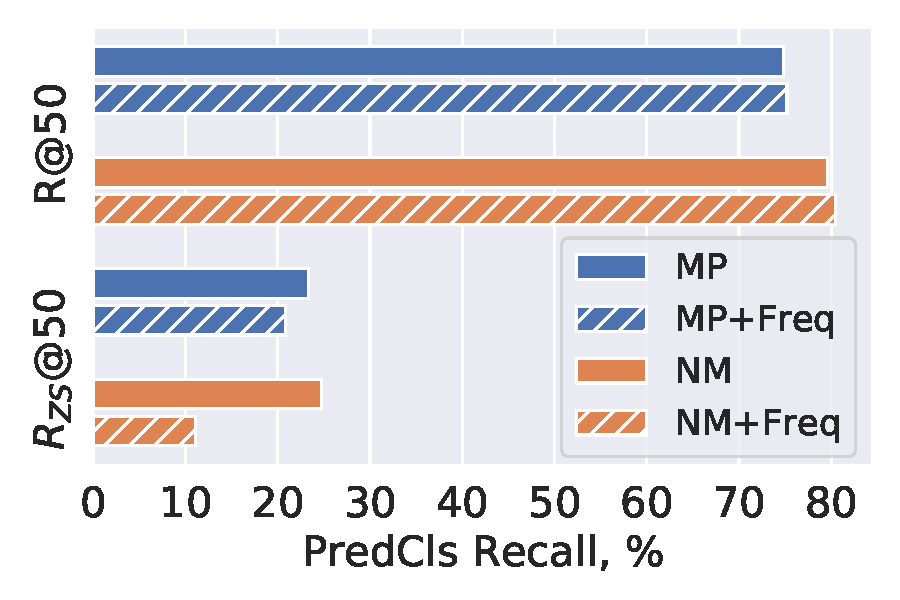
\includegraphics[width=0.4\textwidth,align=c,trim={0.2cm 0 0 0},clip]{freq_bias_vs_ZS.pdf}
	& 
	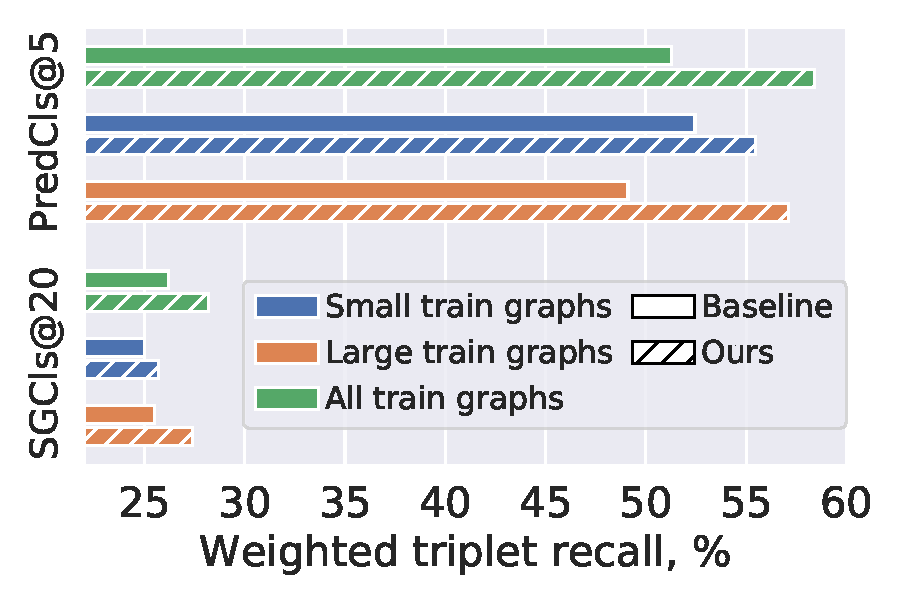
\includegraphics[width=0.4\textwidth,align=c,trim={0.2cm 0 0 0},clip]{large_graphs_vs_loss_norm.pdf}
	%\vspace{-10pt}
	%\caption{\small }\label{fig:results_graph_size}
	\end{tabular}
	%\vspace{-10pt}
	\caption{\small (\textbf{left}) Ablating \textsc{Freq}. \textsc{Freq} only marginally improves results on R@50. At the same time, it leads to large drops in zero-shot recall R$_{ZS}$@50 (and our weighted triplet recall, see Table~\ref{table:main_results}). (\textbf{right}) Learning from small ($N \leq 10$) \textit{vs.}~large ($N>10$) graphs. Our loss makes models learn from larger graphs more effectively, which is important for generalization, because such graphs contain a lot of labels (see \fig{\ref{fig:motivation}}).}\label{fig:freq}
\end{figure}

\vspace{-3pt}
\paragraph{Effect of the Frequency Bias (\textsc{Freq}) on Zero and Few-Shot Performance.}
The \textsc{Freq} model~\citep{zellers2018neural} simply predicts the most frequent predicate between a subject and an object, $P(R|O)$.
Its effect on few-shot generalization has not been empirically studied before. 
We study this by adding/ablating \textsc{Freq} from baseline MP and NM on Visual Genome (\fig{\ref{fig:freq}}, left). Our results show that \textsc{Freq} only marginally improves results on unweighted metrics. At the same time, perhaps unsurprisingly, it leads to severe drops in zero-shot and weighted metrics, especially in NM. For example, by ablating \textsc{Freq} from NM, we improve PredCls-R$_{ZS}$@50 from 11\% to 25\%. This highlights that the existing metrics are a poor choice to measure the effectiveness of a model.\looseness-1

% \begin{wrapfigure}{r}{6.1cm}
% 	\vspace{-45pt}
% 	\centering
	
% 	\vspace{-25pt}
% \end{wrapfigure}

\paragraph{Why does loss normalization help more on few and zero-shots?}
The baseline loss effectively ignores edge labels of large graphs, because it is scaled by a small $d$ in those cases (\fig{\ref{fig:graph_density}}). To validate that, we split the training set of Visual Genome in two subsets, with a comparable number of images in each: with relatively small and large graphs evaluating on the original test set in both cases. We observe that the baseline model does not learn well from large graphs, while our loss enables this learning (\fig{\ref{fig:freq}}, right). Moreover, when trained on small graphs only, the baseline is even better in PredCls than when trained on all graphs. This is because in the latter case, large graphs, when present in a batch, make the whole batch more sparse, downweighting the edge loss of small graphs as well. 
At the same time, larger graphs predictably contain more labels, including many few-shot labels (\fig{\ref{fig:motivation}}). %
Together, these two factors make the baseline ignore many few-shot triplets pertaining to larger graphs at training time, so the model cannot generalize to them at test time.
Since the baseline essentially observes less variability during training, it leads to poor generalization on zero-shots as well. This argument aligns well to the works from other domains~\citep{hill2019environmental}, showing that generalization strongly depends on the diversity of samples during training.
Our loss fixes the issue of learning from larger graphs, which, given the reasons above, directly affects the ability to generalize.\looseness-1


\begin{table}%[]
    \vspace{5pt}
	\scriptsize
	\begin{center}
		\setlength{\tabcolsep}{4pt}
		\begin{minipage}{.46\linewidth}
			%\vspace{-10pt}
			\centering
			\caption{\small{Zero-shot results (R$_{ZS}$@100) on the VTE split~\citep{zhang2017visual}. References: \textsuperscript{1}\citep{zhang2017visual}, \textsuperscript{2}\citep{wang2019generating}, \textsuperscript{3}\citep{yang2018shuffle}, \textsuperscript{4}\citep{wang2019generating}.}}\label{table:zs_comparison_vte}
			\begin{tabular}{lcc}
				\toprule
				\textbf{Model} & \textbf{SGCls-GC} & \textbf{PredCls-GC}\Tstrut\Bstrut\\ 
				\noalign{\smallskip}
				\midrule
				\noalign{\smallskip}
				VTE\textsuperscript{1,2} & $-$ & 16.4 \\
				STA\textsuperscript{3} & $-$ & 18.9 \\
				ST-GAN\textsuperscript{4} & $-$ & 19.0 \\
				MP, baseline~\eqref{eq:loss_baseline} & 2.3 & 20.4 \\
				\noalign{\smallskip}
				\hline
				\noalign{\smallskip}
				MP, ours~\eqref{eq:loss_norm} & \textbf{3.1} & \textbf{21.4} \\
				\bottomrule
			\end{tabular}
		\end{minipage}%
		\hspace{20pt}
		\begin{minipage}{.46\linewidth}
			\setlength{\tabcolsep}{2pt}
			\centering
			\caption{\small {Zero-shot results (R$_{ZS}$@100) on the VG split~\citep{xu2017scene}. \citet{tang2020unbiased} use ResNeXt-101 as a backbone, which helps to improve results.}}\label{table:zs_comparison_vg}
			\begin{tabular}{lcc}
				\toprule
				\textbf{Model} & \textbf{SGCls-GC} & \textbf{PredCls-GC}\Tstrut\Bstrut\\ 
				\noalign{\smallskip}
				%\Xhline{3\arrayrulewidth}
				\midrule
				\noalign{\smallskip}
				NM+TDE~\citep{tang2020unbiased} & \textbf{4.5} & 18.2 \\
				NM, baseline~\eqref{eq:loss_baseline} & 1.7 & 9.5 \\
				MP, baseline~\eqref{eq:loss_baseline} & 3.2 & 20.1 \\
				\noalign{\smallskip}
				\hline
				\noalign{\smallskip}
				NM, ours~\eqref{eq:loss_norm}, no Freq & 3.9 & 20.4 \\
				MP, ours~\eqref{eq:loss_norm} & 4.2 & \textbf{21.5} \\
				\bottomrule
			\end{tabular}
			
		\end{minipage}
		\smallskip \smallskip \smallskip \smallskip \smallskip \smallskip \\
		\caption{\small Comparing our loss to other approaches using MP~\citep{xu2017scene,zellers2018neural} and R/R$_{ZS}$@K metrics. Best results for each metric are bolded.}\label{table:loss_ablations}
		%\vspace{-5pt}
		\setlength{\tabcolsep}{1.2pt}
		\begin{tabular}{l|ll|cc|cc}
			\toprule
			\multicolumn{1}{c|}{} & \multicolumn{2}{c|}{} & \multicolumn{2}{c|}{\textbf{Testing on VG}} & \multicolumn{2}{c}{\textbf{Testing on GQA}}\Tstrut\\
			%\cline{4-7}
			\multirow{1}{*}{\textbf{Tuning dataset}} &
			\multirow{1}{*}{\textbf{Hyperparams}} & 
			\multirow{1}{*}{\textbf{Loss}} & \multicolumn{1}{c}{{SGCls@100}} & \multicolumn{1}{c|}{{PredCls@50}} & \multicolumn{1}{c}{{SGCls@100}} & \multicolumn{1}{c}{{PredCls@50}} \Tstrut\Bstrut\\
			%\Xhline{3\arrayrulewidth}
			\midrule
			No tune (baseline) & $-$ & \eqref{eq:loss_baseline} & 47.2/8.2 & 74.8/23.3 & 27.1/2.8 & 59.7/34.9 \Tstrut \Bstrut\\
			\hline
			VG & $\lambda=20$ & \eqref{eq:loss_tune2} & 48.9/9.2 & \textbf{78.3}/27.9 & 26.6/2.6 & 60.4/36.9 \Tstrut \\
			VG & $\alpha=0.5, \beta=20$ & \eqref{eq:loss_tune1} & \textbf{49.1}/9.4 & 78.2/27.8 & 27.1/2.9 & 60.5/36.3  \\
			GQA & $\lambda=5$ & \eqref{eq:loss_tune2} & 48.8/9.2 & 78.0/26.8 & \textbf{27.8}/2.9 & 60.5/36.1 \\
			GQA & $\alpha=1, \beta=5$ & \eqref{eq:loss_tune1} & 48.6/8.7 & 77.4/27.8 & 27.5/2.9 & 60.7/36.6 \Bstrut \\
			\hline
			No tune (ours, independ. norm) & $\alpha=\beta=1$ & \eqref{eq:loss_tune1} & 47.5/8.4 & 74.3/25.3 & 27.4/2.9 & 59.5/35.4 \Tstrut\\
			No tune (ours, no upweight) & $\gamma=0.05/0.2$ for VG/GQA & \eqref{eq:loss_norm} & 48.7/\textbf{9.6} & \textbf{78.3}/28.2 & 27.4/2.9 & \textbf{61.1}/36.8 \\
			No tune (ours) & $\gamma=1$ & \eqref{eq:loss_norm} & 48.6/9.1 & 78.2/\textbf{28.4} & 27.6/\textbf{3.0} & 61.0/\textbf{37.2} \\
			\bottomrule
		\end{tabular}
	\end{center}
	%\vspace{-5pt}
\end{table}

\paragraph{Alternative approaches.}
We compare our loss to ones with tuned hyperparameters $\alpha,\beta,\lambda$ (Table~\ref{table:loss_ablations}):
\begin{align}
{\cal L} = {\cal L}_{node} + &\alpha {\cal L}_{FG}  + \beta {\cal L}_{BG},\label{eq:loss_tune1} \\
{\cal L} = {\cal L}_{node} + &\lambda {\cal L}_{edge}.\label{eq:loss_tune2}
\end{align}
Our main finding is that, while these losses can give similar or better results in some cases, the parameters $\alpha$, $\beta$ and $\lambda$ do not generally transfer across datasets and must be tuned every time, which can be problematic at larger scale~\citep{zhang2019large}. In contrast, our loss does not require tuning and achieves comparable performance.



To study the effect of density normalization separately from upweighting the edge loss (which is a side effect of our normalization), we also consider downweighting our edge term~\eqref{eq:loss_norm} by some $\gamma<1$ to cancel out this upweighting effect.
This ensures a similar range for the losses in our comparison.
We found (Table~\ref{table:loss_ablations}) that the results are still significantly better than the baseline and, in some cases, even better than our hyperparameter-free loss. This further confirms that normalization of the graph density is important on its own. When carefully fine-tuned, the effects of normalization and upweighting are complimentary (\eg~when $\alpha,\beta$ or $\gamma$ are fine-tuned, the results tend to be better).

\vspace{-6pt}
\paragraph{Comparison to other zero-shot works.}
We also compare to previous works studying zero-shot generalization (Tables~\ref{table:zs_comparison_vte} and~\ref{table:zs_comparison_vg}). %
For comprehensive evaluation, we test on both VTE and VG splits. We achieve superior results on VTE, even by just using the baseline MP, because, as shown in our main results, it generalizes well. On the VG split, we obtain results that compete with a more recent Total Direct Effect (TDE) method~\citep{tang2020unbiased}, even though the latter uses a more advanced detector and feature extractor.
In all cases, our loss improves baseline results and, except for R$_{ZS}$@100 in SGCls, leads to state-of-the-art generalization.
Our loss and TDE can be applied to a wide range of models, beyond MP and NM, to potentially have a complementary effect on generalization, which is interesting to study in future work.


\begin{table}%[]
	%\vspace{-7pt}
	\caption{\small Comparison of our SGG methods to the state-of-the-art on Visual Genome (split~\citep{xu2017scene}). We report results with and without the graph constraint, \textbf{SGGen-GC} and \textbf{SGGen} respectively. %
		All models use Faster R-CNN~\citep{ren2015faster} as a detector, but the models we evaluate use a weaker backbone compared to~\citep{tang2020unbiased}. Interestingly, TDE's improvement on zero-shots (R$_{ZS}$) and mean recall (mR) comes at a significant drop in R@100, which means that frequent triplets are recognized less accurately. Our loss does not suffer from this. Table cells are colored the same way as in Table~\ref{table:main_results}.
		References: \textsuperscript{1}\citep{zellers2018neural},
		\textsuperscript{2}\citep{xu2017scene},
		\textsuperscript{3}\citep{chen2019knowledge},
		\textsuperscript{4}\citep{zhang2019graphical},
		\textsuperscript{5}\citep{tang2020unbiased}. %
	}\label{table:sggen_results}
	\vspace{-10pt}
	\scriptsize
	\setlength{\tabcolsep}{3pt}
	\begin{center}
		\begin{tabular}{llllccccccc} %
			\toprule
			& \multirow{2}{*}{\textbf{Model}} & \multirow{2}{*}{\textbf{Backbone}} & \multirow{2}{*}{\textbf{Loss}} & \multicolumn{3}{c}{\textbf{SGGen-GC}} & &  \multicolumn{3}{c}{\textbf{SGGen}}\Tstrut\Bstrut\\
			\cline{5-7}\cline{9-11}
			& & & & \tiny R@100 & \tiny R$_{ZS}$@100 & \tiny mR@100 & 
			& \tiny R@100 & \tiny R$_{ZS}$@100 & \tiny mR@100 \Tstrut \Bstrut\\
			%\Xhline{2\arrayrulewidth}
			\midrule
			& 
			\textsc{Freq}\textsuperscript{1} & VGG16 & & 27.6 & 0.02 & 5.6 & & 30.9 & 0.1 & 8.9\Tstrut\Bstrut \\
			\cline{2-11}
			& \multirow{3}{*}{MP\textsuperscript{1,2}} & VGG16 & \textsc{Baseline~\eqref{eq:loss_baseline}} & 24.3 & 0.8 & \cellcolor{bad}4.5 & & 27.2 & \cellcolor{bad}0.9 & \cellcolor{bad}7.1\Tstrut \\
			& & VGG16 & \textsc{Ours~\eqref{eq:loss_norm}} & 25.2 & 0.9 & \cellcolor{bad}5.8 & & 28.2 & \cellcolor{bad}1.2 & \cellcolor{bad}9.5\Bstrut\\
			
			& \multirow{3}{*}{NM\textsuperscript{1}} & VGG16 & \textsc{Baseline~\eqref{eq:loss_baseline}} & 29.8 & \cellcolor{extreme}0.3 & \cellcolor{bad}5.9 & & 35.0 & \cellcolor{extreme}0.8 & \cellcolor{bad}12.4\Tstrut \\
			& & VGG16 & \textsc{Ours~\eqref{eq:loss_norm}} & 29.4 & \cellcolor{extreme}1.0 & \cellcolor{bad}\textbf{8.1} & & 35.0 & \cellcolor{extreme}1.8 & \cellcolor{bad}15.4 \\
			& & VGG16 & \textsc{Ours~\eqref{eq:loss_norm}, no Freq} & {30.4} & \cellcolor{extreme}\textbf{1.7} & \cellcolor{bad}7.8 & & {35.9} & \cellcolor{extreme}\textbf{2.4} & \cellcolor{bad}15.3\Bstrut \\
			& KERN\textsuperscript{3} & VGG16 & \textsc{Baseline~\eqref{eq:loss_baseline}} & 29.8 & 0.04 & 7.3 & & 35.8 & 0.02 & \textbf{16.0}\Tstrut\\
			& RelDN\textsuperscript{4} & VGG16 & \textsc{Baseline~\eqref{eq:loss_baseline}} & \textbf{32.7} & $-$ & $-$ & & \textbf{ 36.7} & $-$ & $-$\Bstrut \\
			\cline{2-11}
			& RelDN\textsuperscript{4} & ResNeXt-101 & \textsc{Baseline~\eqref{eq:loss_baseline}} & 36.7 & $-$ & $-$ & & 40.0 & $-$ & $-$\Tstrut \\
			& NM\textsuperscript{5} & ResNeXt-101 & \textsc{Baseline~\eqref{eq:loss_baseline}} & \textbf{36.9} & 0.2 & 6.8 & & $-$ & $-$ & $-$ \\
			& NM+TDE\textsuperscript{5} & ResNeXt-101 & \textsc{Baseline~\eqref{eq:loss_baseline}} & 20.3 & 2.9 & 9.8 & & $-$ & $-$ & $-$  \\
			& VCTree+TDE\textsuperscript{5} & ResNeXt-101 & \textsc{Baseline~\eqref{eq:loss_baseline}} & 23.2 & \textbf{3.2} & \textbf{11.1} & & $-$ & $-$ & $-$\Bstrut \\
			\bottomrule
		\end{tabular}
	\end{center}
	\vspace{-15pt}
	
\end{table}

\vspace{-6pt}
\paragraph{Comparison on SGGen, $P ({\cal G}|I)$.}
In SGCls and PredCls, we relied on ground truth bounding boxes $B_{gt}$, while in SGGen the bounding boxes $B_{pred}$ predicted by a detector should be used to enable a complete image-to-scene graph pipeline. Here, even small differences between $B_{gt}$ and $B_{pred}$ can create large distribution shifts between corresponding extracted features $(V,E)$ (see \secref{\ref{sec:baseline}}), on which SGCls models are trained. Therefore, it is important to \textit{refine} the SGCls model on $(V,E)$ extracted based on predicted $B_{pred}$, according to previous work~\citep{zellers2018neural,chen2019knowledge}. In our experience, this refinement can boost the R@100 result by around 3\% for Message Passing and up to 8\% for Neural Motifs (in absolute terms). In Table~\ref{table:sggen_results}, we report results after the refinement completed both for the baseline loss and our loss in the same way. Similarly to the SGCls and PredCls results, our loss consistently improves baseline results in SGGen. It also allows Neural Motifs (NM) to significantly outperform KERN~\citep{chen2019knowledge} on zero-shots (R$_{ZS}$@100), while being only slightly worse in one of the mR@100 results. The main drawback of KERN is its slow training, which prevented us to explore this model together with our loss. 
Following our experiments in Table~\ref{table:main_results} and \fig{\ref{fig:freq}}, we also confirm the positive effect of removing \textsc{Freq} from NM.
A more recent work of~\citet{tang2020unbiased} shows better results on zero-shots and mean recall, however, we note their more advanced feature extractor, therefore it is difficult to compare our results to theirs in a fair fashion. But, since they also use the baseline loss~\eqref{eq:loss_baseline}, our loss~\eqref{eq:loss_norm} can potentially improve their model, which we leave for future work. 



Finally, we evaluate SGGen on GQA using Message Passing (Table~\ref{table:gqa_sgg}), where we also obtain improvements with our loss. GQA has 1703 object classes compared to 150 in VG making object detection harder. When evaluating SGGen, the predicted triplet is matched to ground truth (GT) if predicted and GT bounding boxes have an intersection over union (IoU) of $\geq$50\%, so more misdetections lead to a larger gap between SGCls and SGGen results.\looseness-1

\begin{table}
	%\vspace{-3pt}
	\centering
	\caption{\small \textbf{SGGen} results on GQA~\citep{hudson2019gqa} using MP. Mask R-CNN~\citep{he2017mask} fine-tuned on GQA is used in this task.}\label{table:gqa_sgg}
	\footnotesize
	\vspace{-3pt}
	%\setlength{\tabcolsep}{1.5pt}
	\begin{tabular}{lccc} 
		%\Xhline{2\arrayrulewidth} 
		\toprule
		\textbf{Loss} & \footnotesize R@300 & \footnotesize R$_{ZS}$@300 &  \footnotesize mR$_{tr}$@300\Bstrut\Tstrut\\
		%\Xhline{2\arrayrulewidth} 
		\midrule
		\textsc{Baseline}~\eqref{eq:loss_baseline} & 6.2 & 0.5 & 1.3 \Tstrut \\ 
		\textsc{Ours}~\eqref{eq:loss_norm}  & \textbf{6.3} & \textbf{0.7} & \textbf{2.4} \Bstrut\\
		\bottomrule 
	\end{tabular}
\end{table} 

%\vspace{-10pt}
\densepar{Qualitative results.}
To qualitatively inspect the effect of our loss on predicted scene graphs, we visualize two cases (\fig{\ref{fig:example}}): (\textbf{top four rows}) when the baseline (MP) model makes a correct prediction, while our model is incorrect; and (\textbf{bottom four rows}) when the baseline is incorrect, while ours is correct. For the purpose of this visualization, a prediction is considered correct when the zero-shot triplet is in the top-20\footnote{Conventionally~\citep{xu2017scene,zellers2018neural}, triplets are ranked according to the product of softmax scores of the subject, object and predicate.} triplets in the image regardless if the detected bounding boxes overlap with the ground truth. In the first case (when the baseline is correct), the predicted triplet often includes the `on' predicate, which we believe is due to the baseline being more biased to the frequency distribution. The model with our loss makes more diverse predictions showing a better understanding of scenes. Also, the ground truth is often mislabeled (see `leaf on bike') or a synonym is predicted by our model (\eg~a plant and a flower), which counts as an error. In the second case (when ours is correct), the baseline model tends to return a poor ranking of triplets and often simply gives a higher rank to frequent triplets. 

\begin{figure}
	\vspace{-10pt}
	\newcommand\Tstrutmore{\rule{0pt}{10ex}}         %
	\newcommand\Bstrutmore{\rule[-2.3ex]{0pt}{0pt}}
	\newcommand{\figwidthvis}{0.14\textwidth}
	\centering
	\tiny
	\setlength{\tabcolsep}{0pt}
	\begin{tabular}{p{0.3cm}|rc|p{0.1cm}rc|p{0.1cm}rc}
		& \multicolumn{2}{c|}{\textsc{Ground truth}} & & \multicolumn{2}{c|}{\textsc{Baseline}} & & \multicolumn{2}{c}{\textsc{Ours}} \\
		& \textsc{Detections} & \textsc{Scene Graph} & & \textsc{Detections} & \textsc{Scene Graph} & & \textsc{Detections} & \textsc{Scene Graph} \\
		\Xhline{5\arrayrulewidth}
		\multirow{8}{*}{\rotatebox[origin=c]{90}{\footnotesize\parbox{6cm}{\vspace{0pt}\textbf{Baseline is correct, Ours is \textcolor{red}{\textbf{incorrect}}}}}} &  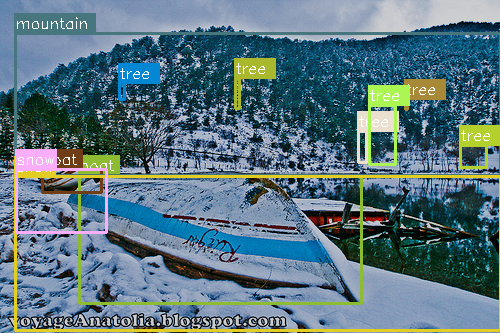
\includegraphics[width=\figwidthvis, align=c]{2337395_baseline_zs.png} &
		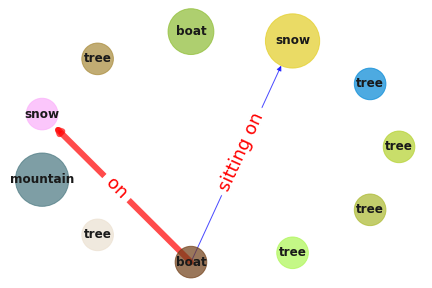
\includegraphics[width=\figwidthvis, align=c]{2337395_baseline_zs_graph_gt.png} & & 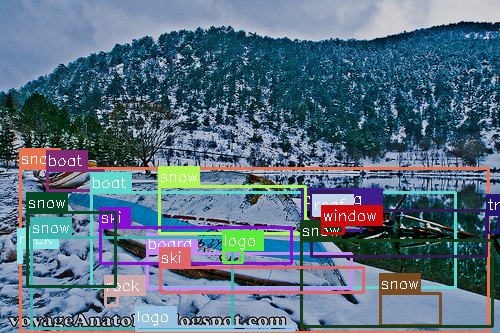
\includegraphics[width=\figwidthvis, align=c]{2337395_baseline_zs_baseline.png} &
		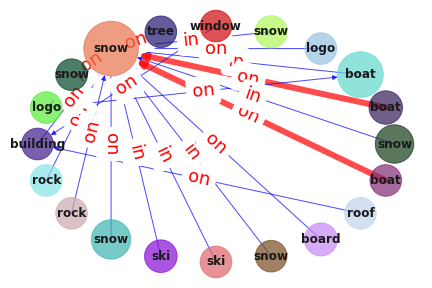
\includegraphics[width=\figwidthvis, align=c]{2337395_baseline_zs_graph_baseline.png} & 
		& 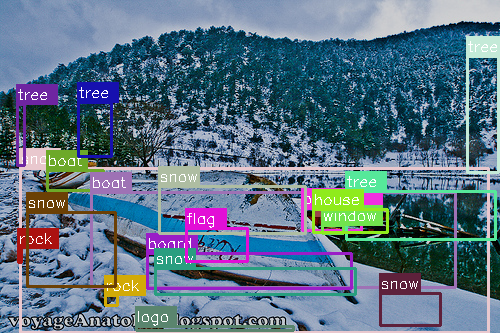
\includegraphics[width=\figwidthvis, align=c]{2337395_baseline_zs_ours.png} & 
		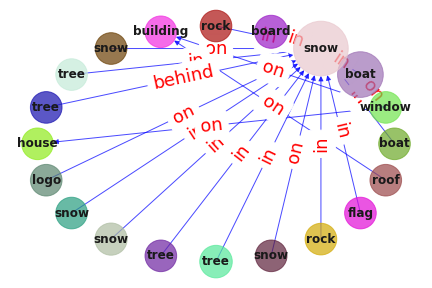
\includegraphics[width=\figwidthvis, align=c]{2337395_baseline_zs_graph_ours.png} \Tstrutmore\Bstrut\\
		& zero-shot triplet: & {boat on snow} & & match: & boat on snow & & closest match: & {boat \textcolor{red}{\textbf{in}} snow} \Bstrut\\
		\cline{2-9} 
		& 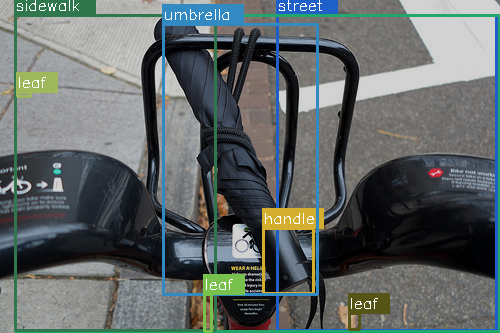
\includegraphics[width=\figwidthvis, align=c]{2412160_baseline_zs.png} &
		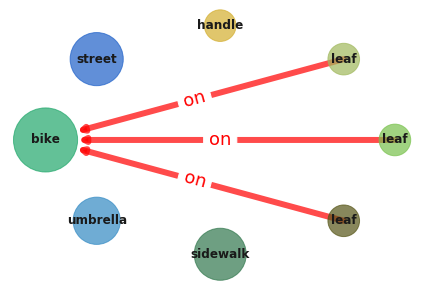
\includegraphics[width=\figwidthvis, align=c]{2412160_baseline_zs_graph_gt.png} & & 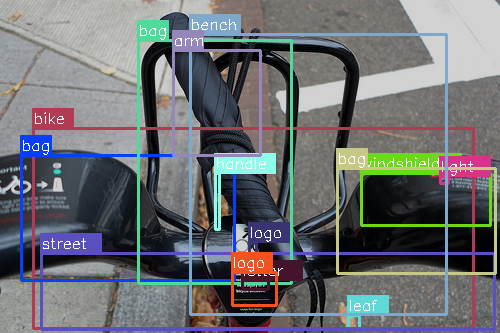
\includegraphics[width=\figwidthvis, align=c]{2412160_baseline_zs_baseline.png} &
		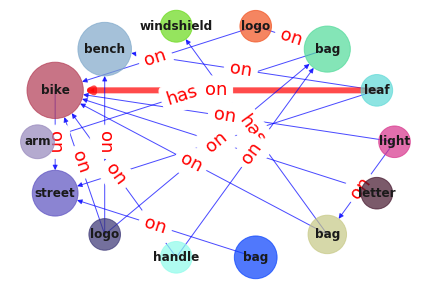
\includegraphics[width=\figwidthvis, align=c]{2412160_baseline_zs_graph_baseline.png} & 
		& 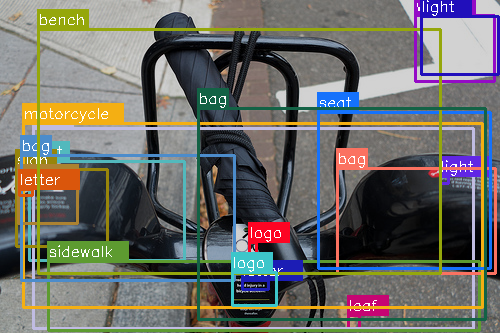
\includegraphics[width=\figwidthvis, align=c]{2412160_baseline_zs_ours.png} & 
		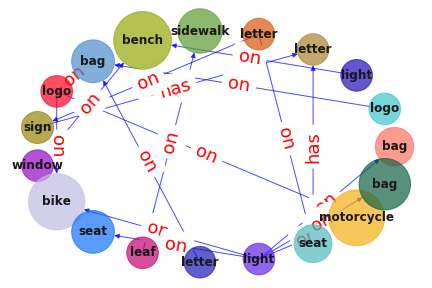
\includegraphics[width=\figwidthvis, align=c]{2412160_baseline_zs_graph_ours.png} \Tstrutmore\Bstrut\\
		& \multicolumn{2}{r|}{zero-shot triplet: \textcolor{violet}{\textbf{leaf on bike}} (mislabeled)} & & match: & leaf on bike & & closest match: & {leaf on \textcolor{red}{\textbf{sidewalk}}} \Bstrut\\
		\cline{2-9} 
		& 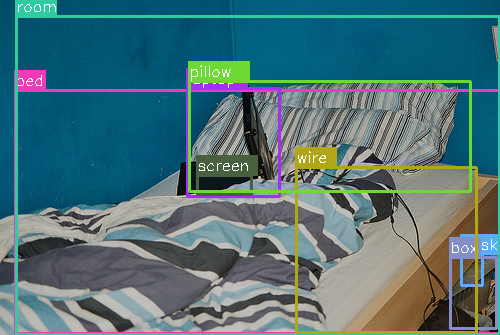
\includegraphics[width=\figwidthvis, align=c]{2326876_baseline_zs.png} &
		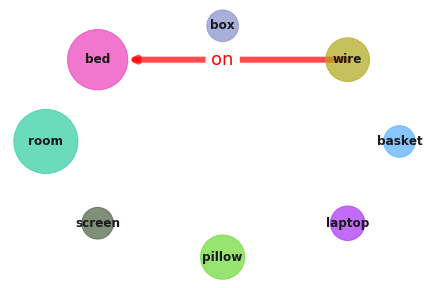
\includegraphics[width=\figwidthvis, align=c]{2326876_baseline_zs_graph_gt.png} & & 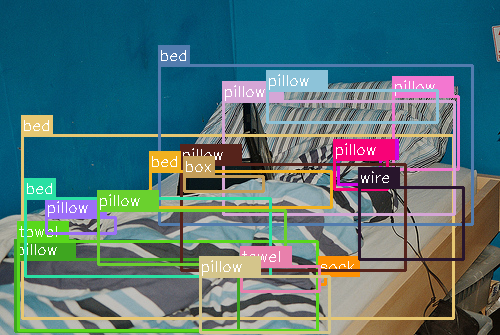
\includegraphics[width=\figwidthvis, align=c]{2326876_baseline_zs_baseline.png} &
		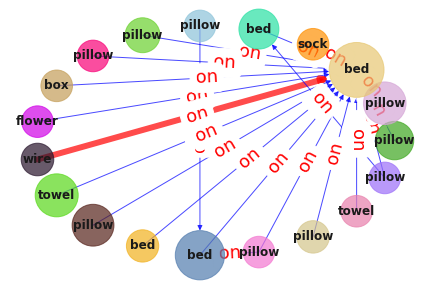
\includegraphics[width=\figwidthvis, align=c]{2326876_baseline_zs_graph_baseline.png} & 
		& 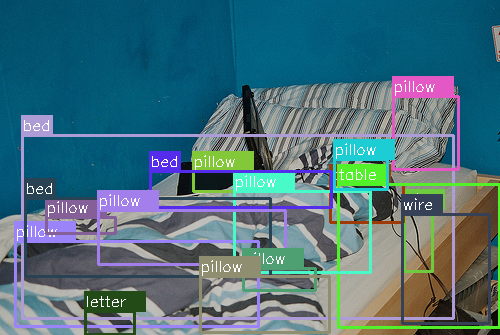
\includegraphics[width=\figwidthvis, align=c]{2326876_baseline_zs_ours.png} & 
		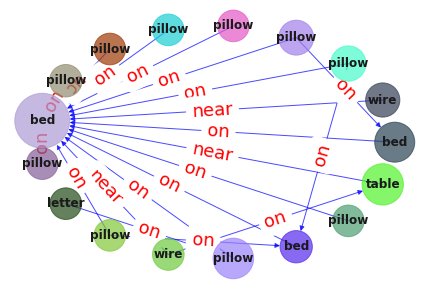
\includegraphics[width=\figwidthvis, align=c]{2326876_baseline_zs_graph_ours.png} \Tstrutmore\Bstrut\\
		& zero-shot triplet: & {wire on bed} & & match: & wire on bed & & closest match: & {wire \textcolor{red}{\textbf{near}} bed} \Bstrut\\
		\cline{2-9} 
		& 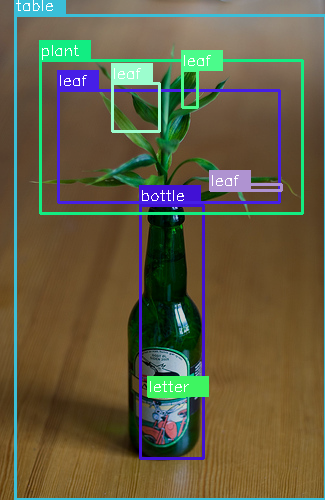
\includegraphics[width=\figwidthvis, height=1.8cm, align=c]{2315538_baseline_zs.png} &
		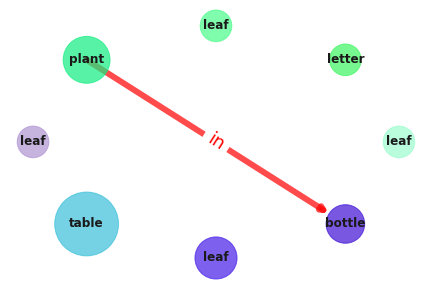
\includegraphics[width=\figwidthvis, align=c]{2315538_baseline_zs_graph_gt.png} & 
		& 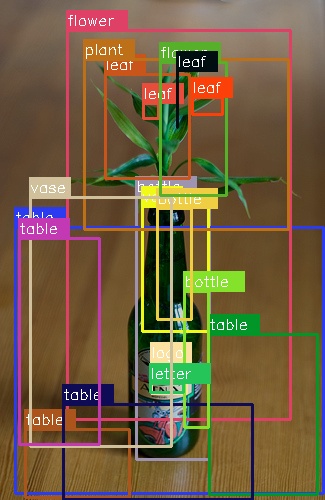
\includegraphics[width=\figwidthvis, height=1.8cm, align=c]{2315538_baseline_zs_baseline.png} &
		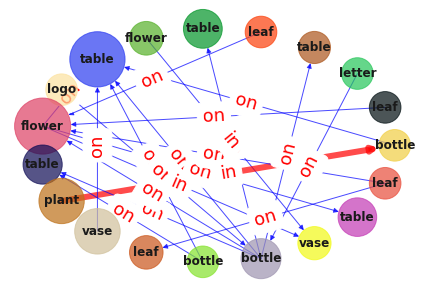
\includegraphics[width=\figwidthvis, align=c]{2315538_baseline_zs_graph_baseline.png} & 
		& 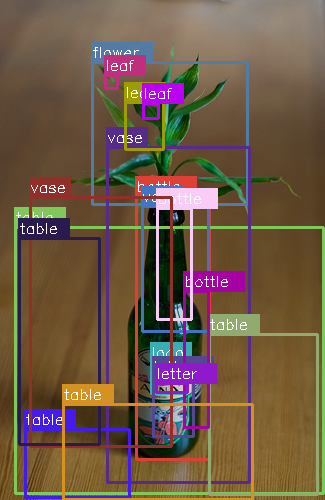
\includegraphics[width=\figwidthvis, height=1.8cm, align=c]{2315538_baseline_zs_ours.png} &
		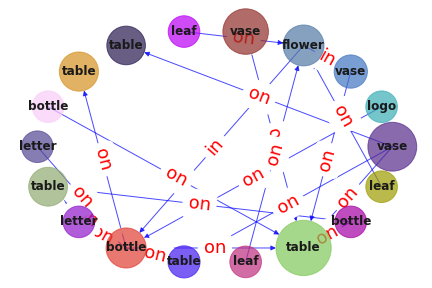
\includegraphics[width=\figwidthvis, align=c]{2315538_baseline_zs_graph_ours.png} \Tstrutmore\Bstrut\\
		& zero-shot triplet: & {plant in bottle} & & match: & plant in bottle & & closest match: & {\textcolor{red}{\textbf{flower}} in bottle}\Bstrut\\
		
		\Xhline{5\arrayrulewidth}
		\multirow{8}{*}{\rotatebox[origin=c]{90}{\footnotesize\parbox{6cm}{\textbf{Baseline is \textcolor{red}{\textbf{incorrect}}, Ours is correct}}}} &
		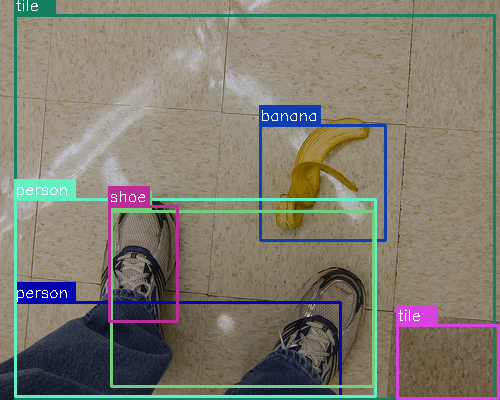
\includegraphics[width=\figwidthvis, height=1.8cm, align=c]{2317051_ours_zs.png} &
		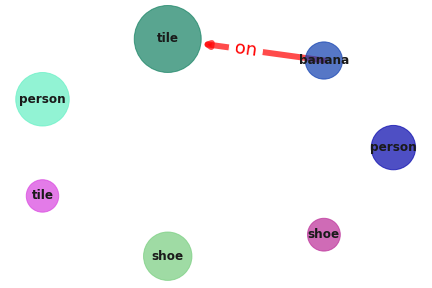
\includegraphics[width=\figwidthvis, align=c]{2317051_ours_zs_graph_gt.png} & &  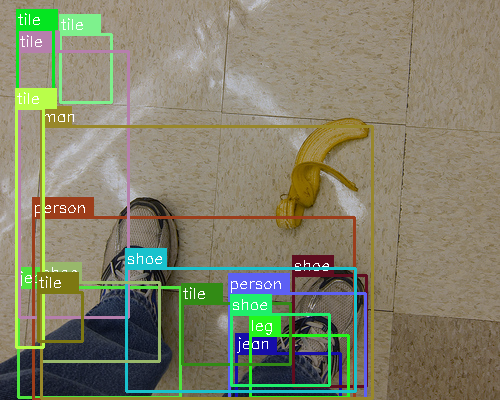
\includegraphics[width=\figwidthvis, height=1.8cm, align=c]{2317051_ours_zs_baseline.png} &
		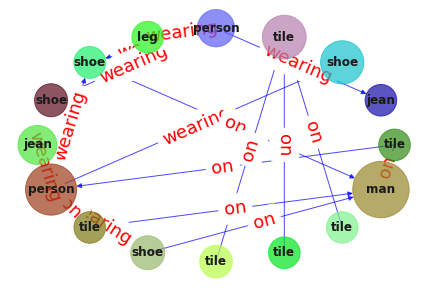
\includegraphics[width=\figwidthvis, align=c]{2317051_ours_zs_graph_baseline.png} & 
		& 
		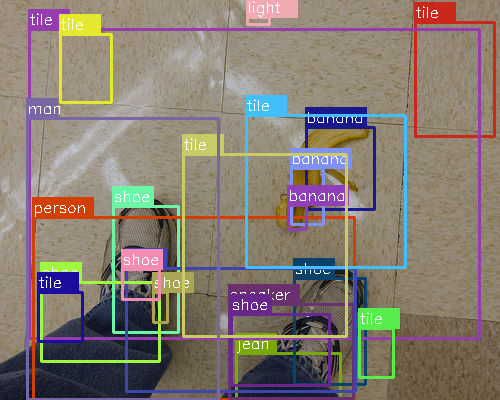
\includegraphics[width=\figwidthvis, height=1.8cm, align=c]{2317051_ours_zs_ours.png} & 
		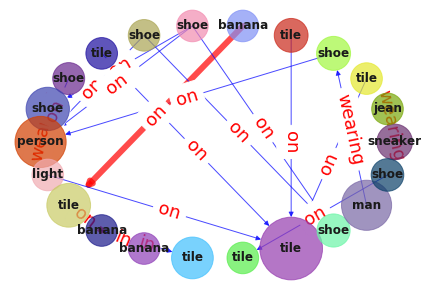
\includegraphics[width=\figwidthvis, align=c]{2317051_ours_zs_graph_ours.png} \Tstrutmore\Bstrut\\
		& zero-shot triplet: & {banana on tile} & & \multicolumn{2}{r|}{no triplet involving a banana in top-20} & & match: & {banana on tile} \Bstrut\\
		\cline{2-9} 
		& 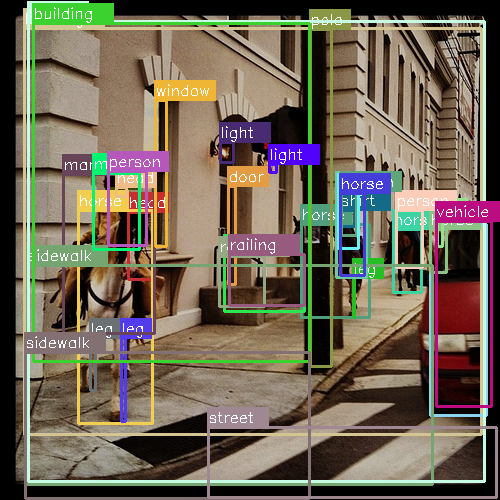
\includegraphics[width=\figwidthvis, height=1.8cm, align=c]{2320180_ours_zs.png} &
		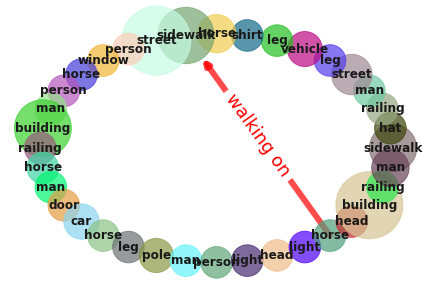
\includegraphics[width=\figwidthvis, align=c]{2320180_ours_zs_graph_gt.png} & & 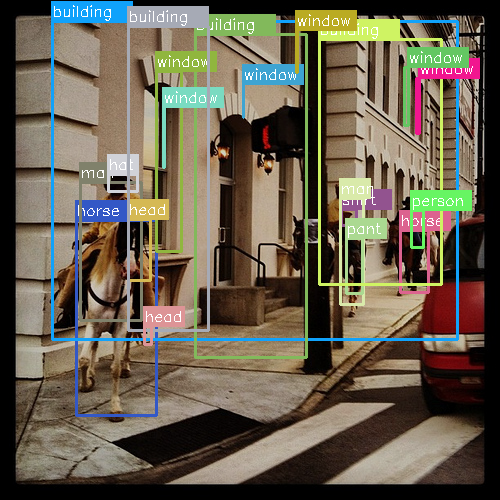
\includegraphics[width=\figwidthvis, height=1.8cm, align=c]{2320180_ours_zs_baseline.png} &
		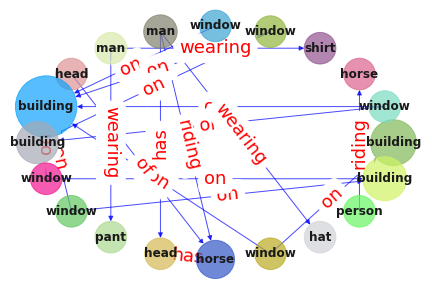
\includegraphics[width=\figwidthvis, align=c]{2320180_ours_zs_graph_baseline.png} & 
		& 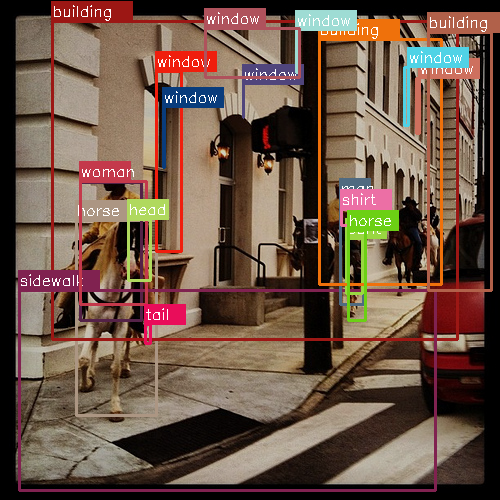
\includegraphics[width=\figwidthvis, height=1.8cm, align=c]{2320180_ours_zs_ours.png} & 
		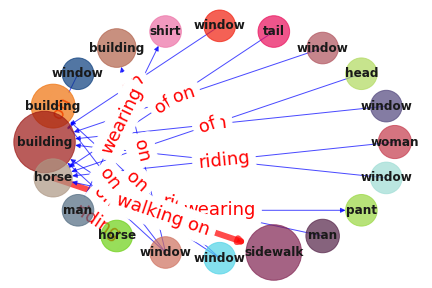
\includegraphics[width=\figwidthvis,align=c]{2320180_ours_zs_graph_ours.png} \Tstrutmore\Bstrut\\
		& \multicolumn{2}{r|}{zero-shot triplet: horse walking on sidewalk} & & \multicolumn{2}{r|}{no triplet involving a sidewalk in top-20} & & \multicolumn{2}{r}{match: horse walking on sidewalk} \Bstrut\\
		\cline{2-9}  
		& 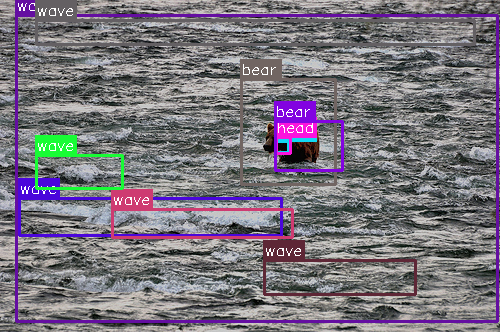
\includegraphics[width=\figwidthvis, align=c]{2334137_ours_zs.png} &
		\includegraphics[width=\figwidthvis, align=c]{2334137_ours_zs_graph_gt.png} & & \includegraphics[width=\figwidthvis, align=c]{2334137_ours_zs_baseline.png} &
		\includegraphics[width=\figwidthvis, align=c]{2334137_ours_zs_graph_baseline.png} & 
		& \includegraphics[width=\figwidthvis, align=c]{2334137_ours_zs_ours.png} & 
		\includegraphics[width=\figwidthvis, align=c]{2334137_ours_zs_graph_ours.png} \Tstrutmore\Bstrut\\
		& zero-shot triplet: & {bear in wave} & & closest match: & bear \textcolor{red}{\textbf{on}} wave & & match: & bear in wave \Bstrut\\
		\cline{2-9} 
		& \includegraphics[width=\figwidthvis, height=1.8cm, align=c]{2320504_ours_zs.png} &
		\includegraphics[width=\figwidthvis, align=c]{2320504_ours_zs_graph_gt.png} & & \includegraphics[width=\figwidthvis, height=1.8cm, align=c]{2320504_ours_zs_baseline.png} &
		\includegraphics[width=\figwidthvis, align=c]{2320504_ours_zs_graph_baseline.png} & 
		& 
		\includegraphics[width=\figwidthvis, height=1.8cm, align=c]{2320504_ours_zs_ours.png} & 
		\includegraphics[width=\figwidthvis, align=c]{2320504_ours_zs_graph_ours.png} \Tstrutmore\Bstrut\\
		& zero-shot triplet: & {woman sitting on rock} & & \multicolumn{2}{r|}{no triplet involving a rock in top-20} & & \multicolumn{2}{r}{match: woman sitting on rock}\\
		\hline
	\end{tabular}
	\vspace{-5pt}
	\caption{\small Visualizations of scene graph generation for zero-shots (denoted as thick red arrows) on Visual Genome using Message Passing with the baseline loss versus our loss. Most edges are two-way, but for clarity we show them one-way.
		{These examples are picked randomly. Intended to be viewed on a computer display.}}
	\label{fig:example}
\end{figure}

%\vspace{-5pt}
\section{Conclusions}
\vspace{-8pt}

Scene graphs are a useful semantic representation of images, accelerating research in many applications including visual question answering.
It is vital for the SGG model to perform well on rare/unseen compositions of objects and predicates, which are inevitable due to an extremely long tail of the distribution over triplets. We show that baseline models do not effectively learn from all labels, leading to poor generalization on few/zero shots. Moreover, current evaluation metrics do not reflect this problem, exacerbating it instead.
We also show that learning well from larger graphs is essential to enable stronger generalization. To this end, we modify the loss commonly used in SGG and achieve significant gains and, in certain cases, state-of-the-art results, on both the existing and our novel weighted metric.\looseness-1
